
%----------------------------------------------------------------------------
\documentclass[a4paper,11pt]{article} 
%----------------------------------------------------------------------------

%----------------------------------------------------------------------------
%% Language and font encodings
%----------------------------------------------------------------------------
\usepackage[a4paper,top=3cm,bottom=2cm,left=3cm,right=3cm,marginparwidth=1.75cm]{geometry}
\usepackage{graphicx} 
\usepackage[hidelinks]{hyperref} 
\usepackage{multirow} 
\usepackage{tabularx} 
\usepackage{color} 

\usepackage[fleqn]{amsmath}
\usepackage{amsfonts}
\usepackage{amssymb}
\usepackage{textcomp}
\usepackage{gensymb}

\usepackage{array}

\setlength\parindent{0pt}

\usepackage{amsxtra} 

\usepackage{wasysym} 
\usepackage{isomath} 
\usepackage{mathtools} 
\usepackage{txfonts} 
\usepackage{upgreek} 
\usepackage{enumerate} 
\usepackage{tensor} 
\usepackage{pifont} 
\usepackage{titlesec}

\usepackage[utf8x]{inputenc}
\usepackage[T1]{fontenc}
\usepackage{fancyhdr}
%\usepackage{enumitem}
%\usepackage[colorlinks=true, allcolors=blue]{hyperref}
\usepackage{subcaption}

\usepackage[normalem]{ulem} %25/05
\usepackage{caption}%04/06
\usepackage{afterpage}%04/6

\usepackage{geometry}%05/06

\usepackage{wrapfig}%04/06
\usepackage{float}
%\usepackage[printfigures]{endfloat}
%\usepackage{endfloat}
%\usepackage{subfig}
%\usepackage{graphicx}
%package floatend

%----------------------------------------------------------------------------
% Packages: uncomment to debug
%----------------------------------------------------------------------------
%\usepackage{refcheck}
%\renewcommand{\labelitemi}{\textbullet}

%----------------------------------------------------------------------------
% Packages: bibliography
%----------------------------------------------------------------------------
\usepackage[nottoc, notlof, notlot]{tocbibind}
%\usepackage[authoryear, round]{natbib}
\usepackage[authoryear]{natbib}

\usepackage[english]{babel}

\usepackage{authblk}

%----------------------------------------------------------------------------
% Colors...
%----------------------------------------------------------------------------
\definecolor{color-1}{rgb}{0.21,0.37,0.57}
\definecolor{color-2}{rgb}{0.31,0.51,0.74}

%----------------------------------------------------------------------------
\titleformat*{\section}{\large\bfseries}
\titleformat*{\subsection}{\normalfont\bfseries}
\title{Modified Acoustic, Internadeepl and Surface Waves and Modes in the Ocean}

%----------------------------------------------------------------------------
\geometry{hmargin=2.5cm,vmargin=2.5cm} %marges
%----------------------------------------------------------------------------


%%%%%%%%%%%%%%%%%%%%%%%%%%%%%%%%%%%%%%%%%%%%%%%%%%%%%%%%%%%%%%%%%%%%%%%%%%%
\author[1]{F. Auclair\thanks{Corresponding author: francis.auclair@aero.obs-mip.fr}}
\author[2]{X. Capet}
\author[3]{L. Debreu}
\author[4]{F. Dumas}
\author[1]{M. Hilt}
\author[5]{P. Marchesiello}
\author[1]{C. Nguyen}
\author[1]{L. Roblou}
%
%\author[affilINRIA]{F. Lemari\'e}
%\author[affilIFREMER]{S. Jullien}
%\author[affilSHOM]{L. Bordois}
%\author[affilLEGOSCNRS]{R. Benshila}
%
\affil[1]{Laboratoire d'A\'erologie, Universit\'e de Toulouse, CNRS, UPS, France}
\affil[2]{IPSL/LOCEAN, CNRS, 
UPMC, IRD, MNHN, France}
\affil[3]{Univ Grenoble Alpes, Inria, CNRS, 38000 Grenoble INP, LJK, Grenoble, France}
\affil[4]{Service Hydrographie et Oc\'eanographie de la Marine, Brest, France}
\affil[5]{LEGOS, IRD, Universit\'e de Toulouse, CNRS, CNES, France}
%
%\address[affilLEGOSCNRS]{LEGOS/CNRS, 31400 Toulouse, France}
%\address[affilIFREMER]{Ifremer, Univ. Brest, CNRS, IRD, Laboratoire d'Océanographie Physique et Spatiale (LOPS), IUEM, F- 29280, Plouzan\'e, France}
%
%%%%%%%%%%%%%%%%%%%%%%%%%%%%%%%%%%%%%%%%%%%%%%%%%%%%%%%%%%%%%%%%%%%%%%%%%%%

%%%%%%%%%%%%%%%%%%%%%%%%%%%%%%%%%%%%%%%%%%%%%%%%%%%%%%%%%%%%%%%%%%%%%%%%%%%%
\begin{document}
%%%%%%%%%%%%%%%%%%%%%%%%%%%%%%%%%%%%%%%%%%%%%%%%%%%%%%%%%%%%%%%%%%%%%%%%%%%%%
%\bibliographystyle{agsm}

\renewcommand{\thepage}{}
\hypersetup{pdfborder=0 0 0}
\maketitle
\setcounter{tocdepth}{2}

%----------------------------------------------------------------------------
% \ref with ( )
%----------------------------------------------------------------------------
\let\oldref\ref
\renewcommand{\ref}[1]{(\oldref{#1})}

%%%%%%%%%%%%%%%%%%%%%%%%%%%%%%%%%%%%%%%%%%%%%%%%%%%%%%%%%%%%%%%%%%%%%%%%%%%%%
%\tableofcontents
%%%%%%%%%%%%%%%%%%%%%%%%%%%%%%%%%%%%%%%%%%%%%%%%%%%%%%%%%%%%%%%%%%%%%%%%%%%%%

%%%%%%%%%%%%%%%%%%%%%%%%%%%%%%%%%%%%%%%%%%%%%%%%%%%%%%%%%%%%%%%%%%%%%%%%%%%%%
% Abstract
%%%%%%%%%%%%%%%%%%%%%%%%%%%%%%%%%%%%%%%%%%%%%%%%%%%%%%%%%%%%%%%%%%%%%%%%%%%%%
\textit{Abstract:} waves can propagate in a free-surface ocean due to compressibility or gravity and, at much lower scale, due to surface tension. Analytical solutions have for long been derived independently for acoustic waves or internal-gravity rays (in an unbounded ocean), for surface-gravity waves (in a free-surface-ocean) and for acoustic or internal modes (in a bounded ocean). In the present study, capillarity waves and earth-rotation are neglected and a simple, unified model based on two dispersion relations is derived for waves propagating in a compressible, stratified, free-surface ocean. This model is an extension of Dukowicz's (\cite{dukowicz_2013}). Wave solutions are first identified and carefully studied geometrically in phase-space. Taylor developments are then carried out with respect to small parameters describing stratification and compressibility and are compared to numerical approximations of the intersection of the various branches of the inner and boundary dispersion surfaces. Known approximations for swell, long-surface waves, internal-gravity rays, internal modes, acoustic waves or acoustic modes are recovered and perturbations due to ocean stratification and/or compressibility are discussed.\\

%%%%%%%%%%%%%%%%%%%%%%%%%%%%%%%%%%%%%%%%%%%%%%%%%%%%%%%%%%%%%%%%%%%%%%%%%%%
\newpage
\renewcommand{\thepage}{\arabic{page}}
\setcounter{page}{1}
%%%%%%%%%%%%%%%%%%%%%%%%%%%%%%%%%%%%%%%%%%%%%%%%%%%%%%%%%%%%%%%%%%%%%%%%%%%%%
\section{Introduction}
%%%%%%%%%%%%%%%%%%%%%%%%%%%%%%%%%%%%%%%%%%%%%%%%%%%%%%%%%%%%%%%%%%%%%%%%%%%%%
Many types of waves are known to propagate in the ocean and textbooks (\cite{LeBlond_Mysak_1981}; \cite{gill_1982}; \cite{Pedlosky_1982}...) have for long detailed the derivation of analytical solutions. These waves can basically be classified in several categories depending on the type of mechanisms directly involved in their propagation. Neglecting modification due to rotation for no-so-long waves, two fundamental categories are of particular interest in the present study: acoustic (or sound) waves which are a consequence of the compressibility of the ocean and gravity waves which are sustained by the gravity force. Table \ref{TableWave solutions} gives a short (and necessarily incomplete) list of such waves together with their dispersion relations. Acronyms for the corresponding modified waves studied below are indicated in the last column. The names, the dispersion relations and the parametrized relations are indicated in Table \ref{TableWaveAcronyms}. A particular wave is indeed most often described by giving one or a few space-time \textit{dispersion} relations linking for instance its pulsation (or its period) to its wave-numbers (or to its wave-lengths). Its phase and group velocities and several physical properties such as its capacity to "disperse" wave-lengths can be derived from the dispersion relations.\\
In the ocean, if the wavelengths are small enough and if they are generated far enough from the surface and bottom boundaries, these waves can propagate as in any unbounded medium. However, when they are generated in the vicinity of these boundaries or when their wavelengths are large compared to the ocean depth, waves are known to take particular forms and the ocean can then be assimilated to a \textit{wave-guide} propagating \textit{wave-modes}. Internal (gravity) mode solutions with "long" horizontal wavelengths have for long been known to propagate in the ocean wave-guide and acoustic wave-mode solutions have lately been re-discovered by Smith (\cite{smith_2015}). These internal and acoustic waves are qualified as "wave modes" due to the quantification of their vertical wavelength.\\
The ocean free-surface is permanently shaken by a myriad of horizontally propagating waves and it is not always very clear if these waves are wave-modes or just vertically-evanescent edge-waves. Capillary waves (not studied here), swells, tidal waves, tsunamis are well-known examples.\\
Deriving a dispersion relation for acoustic waves or for internal wave rays in an unbounded ocean is rather straightforward. The proposed method generally includes two steps: firstly, waves are supposed to have very small amplitude and, secondly, only the specific wave-restoring mechanisms and medium characteristics are retained in an as-simple-as-possible wave dispersion model (compressibility and pressure force for acoustic waves, gravity and vertical advection of isopycnal surfaces for internal waves). The linear nature of the resulting model has two main advantages: analytical solutions can be carried out and waves can be superimposed without interacting (\cite{lighthill_1967}).
The treatment of the free-surface boundary can yet be much trickier: small-amplitudes are usually postulated and both gravity and free-surface motions are retained in the dedicated dispersion model. However, surface waves are "edge waves" propagating at the interface between the atmosphere and the ocean meaning that the surface kinematic relation (the free-surface general boundary-condition) leads to a transcendental dispersion relation with trigonometric terms. This obviously results in difficulties to derive analytical solutions for ocean surface waves and it requires, in any case, further simplifications. Numerous specific analytical solutions can then be found in the literature depending for instance on the ratio of the horizontal wavelength to the ocean depth $(H)$ (Table \oldref{TableWave solutions}). Long gravity surface wave solutions can indeed be found with small such ratios and these waves are well-known to propagate horizontally with $\sqrt{g H}$ phase and group velocities (with g the acceleration of gravity).\\

%%%%%%%%%%%%%%%%%%%%%%%%%%%
% Table  Wave solutions
%%%%%%%%%%%%%%%%%%%%%%%%%%%
\newcolumntype{P}[1]{>{\centering\arraybackslash}p{#1}}
\begin{table}[!h]
	\setlength{\extrarowheight}{15pt}
	\begin{tabular} {P{2.7cm}|P{3cm}|c|P{2.3cm}|P{3cm}}
		Waves & Assumptions & Pulsation $(\Omega)$ & $k_z$ & Modified wave\\\hline
		Acoustic waves & Compressible, unbounded &$\Omega_{aw}^2=c_s^2(k_x^2+k_z^2)$& & MAW \\
		Internal gravity rays & Stratified, unbounded &$\Omega_{iwr}^2=\frac{N^2 k_x^2}{k_x^2+k_z^2}$ & & MIW \\\hline
		Acoustic gravity modes & Compressible, bounded &$\Omega_{am}^2=c_s^2(k_x^2+k_z^2)$&$k_{z,am}=\frac{\pi}{2H}+\frac{m\pi}{H}$ & MAM \\
		Swell & Free-surface &$\Omega_{sw}^2=g k_x tan(k_x H)$ &$k_{z,sw}\approx k_x$ & MSW \\
		Long Surface waves & Free-surface, shallow &$\Omega_{lsw}^2=gH\ k_x^2$ &$k_{z,lsw}\approx k_x$& LMSW \\
		Internal gravity modes & Stratified, bounded &$\Omega_{im}^2=\frac{N\pi}{nH}$&$k_{z,im}=\frac{n\pi}{H}$ & MIMn \\
		Low frequency Oscillations
		(Long MIM, $n=0$) & Stratified, bounded & & & LMIM0\\
	\end{tabular}
	
	\caption{examples of ocean waves and their dispersion relations in a vertical section. $\Omega$ is the pulsation of the wave, $k_x$ and $k_z$ are the wave-numbers, $g$ is the acceleration of gravity, $H$ a reference depth, $N$ a reference Brun-Väisälä pulsation and $c_s$ the speed of sound. $n$ and $m$ are two positive integer numbers.}
	\label{TableWave solutions}
\end{table}
%%%%%%%%%%%%%%%%%%%%%%%%%%%
% Table 
%%%%%%%%%%%%%%%%%%%%%%%%%%%


%%%%%%%%%%%%%%%%%%%%%%%%%%%
% Table  AGWaves acronyms 22222
%%%%%%%%%%%%%%%%%%%%%%%%%%%
\newcolumntype{P}[1]{>{\centering\arraybackslash}p{#1}}
\begin{table}[!h]
	\setlength{\extrarowheight}{15pt}
	\begin{tabular} {c|c|c|c}
		Acronym & Name & Dispersion relations & Parametrized relations \\\hline
		MAW & Modified Acoustic Wave & \ref{DispAcousDT} & MAW \ref{DispAcousDT}\\
		MIW & Modified Internal Wave ray & \ref{DispRaysDT} & MIW \ref{DispRaysDT}\\\hline
		MAM & Modified Acoustic Mode $(m=1)$& (\oldref{EqFullDispera} \& \oldref{EqFullDisperb}) & MAM (\oldref{paramMAM1}, \oldref{paramMAM2}),\\
		& & & LMAM (\oldref{ParamLMAM1}, \oldref{ParamLMAM2})\\
		MSW & Modified Surface Wave & \ref{EqFullDisperai} \& \ref{EqFullDisperb} & MSW (\oldref{EqDispLonga1} \& \oldref{Eqdzdx2}) \\
		LMSW & Long Modified Surface Wave & \ref{EqFullDisperai} \& \ref{EqFullDisperb} & LMSW (\oldref{Eqxxx} \& \oldref{EqDispDeltaz0}) \\
		MIM & Modified Internal Mode $(n=1)$  & (\oldref{EqFullDispera} \& \oldref{EqFullDisperb}) & MIM (\oldref{ParamallMIM1}, \oldref{ParamallMIM2}),\\
		& & & LMIM (\oldref{ParamMIM1}, \oldref{ParamMIM2})\\
		LMIM0 & Long Gravity Oscillation (LMIM 0)& \ref{EqFullDispera} \& \ref{Eqxxx} & LMIM0 (\oldref{MIMomega2}, \oldref{MIMdz2})\\
	\end{tabular}
	
	\caption{Acronyms of modified wave and modes.}
	\label{TableWaveAcronyms}
\end{table}
%%%%%%%%%%%%%%%%%%%%%%%%%%%
% Table 
%%%%%%%%%%%%%%%%%%%%%%%%%%%

Such simplified models for small-amplitude waves are facing (at least) two severe limitations when compared to real-life ocean waves. Firstly, real ocean waves do not have an infinitesimal amplitude and finite-amplitude waves differ from their small-amplitude avatars: their non-linear growth can indeed lead to breaking or to new equilibrium when non-linearity can be counteracted by wave dispersion (propagating for instance as solitary waves). The second limitation comes from the fact that only specific wave-restoring mechanisms and medium characteristics are retained in process-oriented dispersion models whereas, in real ocean, compressibility can modify internal and surface waves and gravity can modify acoustic waves. Mixed acoustic-gravity waves can also be expected to propagate in the ocean.\\
Dukowicz (2013) tackled with this problem and proposed a review of the \textit{"various approximations in atmosphere and ocean model based on an exact treatment of gravity wave dispersion"}. In the ocean, acoustic-gravity waves are shown by the author to satisfy a system of two dispersion relations and the impact of several usual assumptions often made in ocean models is evaluated. The present study builds on Dukowicz's study and more specifically focuses on the consequences of both the stratification and compressibility of the ocean on the properties of acoustic-gravity waves and wave-modes: Taylor expansions of dispersion relations and of the many resulting expressions for wavelengths and pulsation are derived in terms of both compressibility and stratification. In addition:
\begin{itemize}
	\item We show that free-surface boundary constraints can be recovered at the same order of precision as in Dukowicz's but using an Eulerian framework. We do not intent to show that the Eulerian framework makes more physical sense than the Lagrangian framework but just that it can reduce the analytical burden.
	\item A systematic graphic investigation of wave solutions is carried out in (3D) pulsation/wave-number phase-space, unfolding and investigating the dependency to the vertical wave-number compared to Dukowicz' study. Graphic explorations give an overall idea of the possible connections between the usual acoustic, internal and surface wave solutions.
	\item Surface waves (edge waves in Dukowicz's denomination) together with internal and acoustic wave-modes are systematically studied in the ocean. "Acoustic-gravity" wave modes (\cite{smith_2015}) are in particular recovered in the same general framework. 
	\item Long-wave solutions are investigated in details in order to better understand from which solution branch they asymptotically derive and approximate parametric relations are systematically derived for each type of wave.
	\item A particular region of phase space is identified where surface acoustic-gravity surface wave are "structurally singular" in the sense that gravity and compressiblity are both important and the corresponding wave solution is close to instability in time.
\end{itemize}   
On some of these points, our conclusions can either extend, confirm or, on the contrary, contradict the conclusions drawn by Dukowicz.\\
In the following section \ref{SectionLinModels}, a linear model of wave propagation is proposed for the ocean together with bottom and surface boundary conditions and a system of two dispersion relations is derived from this model. The inner dispersion relation is studied in details in the following section \ref{SectionInner} and the wave solutions propagating in an unbounded ocean are investigated. Wave propagating in a bounded ocean are then studied in section \ref{SectionGraphic}. The resulting solutions are further discussed in a last section \ref{SectionDiscussion}.

%\newpage
%\textit{Objectives and novelty of the present study:}
%\begin{itemize}
%	\item general dispersion relations for acoustic and gravity waves,
%	\item modification of gravity (acoustic) waves by
%	\item (i) graphical study and identification of various wave solutions,
%	\item (ii) Taylor expansion of the inner and surface relations to compute wave solutions,
%	\item (iii) Taylor expansion of the identified wave solutions in terms of non-linearity and non-hydrostaticity.
%	\item tan and tanh surface solutions (transcendental).
%	\item analytical solutions in $\omega$ of the inner ocean dispersion relation.
%	\item comparison with classical solution.
%	\item numerical solutions of the intersections.
%\end{itemize}


%%%%%%%%%%%%%%%%%%%%%%%%%%%%%%%%%%%%%%%%%%%%%%%%%%%%%%%%%%%%%%%%%%%%%%%%%%%%%
\newpage
%%%%%%%%%%%%%%%%%%%%%%%%%%%%%%%%%%%%%%%%%%%%%%%%%%%%%%%%%%%%%%%%%%%%%%%%%%%%%
\section{Linear Model for surface and internal acoustic-gravity waves}
\label{SectionLinModels}
%%%%%%%%%%%%%%%%%%%%%%%%%%%%%%%%%%%%%%%%%%%%%%%%%%%%%%%%%%%%%%%%%%%%%%%%%%%%%

\subsection{General model for a compressible, viscous ocean}
\label{SubSectionNSModel}
Ocean dynamics can be described with a small number of macroscopic variables: its velocity $(\vec{v})$, its pressure and density ($p$ and $\rho$), its temperature and salinity ($T$ and $S$).
In a Cartesian framework, the general equations governing the motion of a compressible, viscous ocean are then:
\begin{subequations}
 \begin{alignat}{2}
 \displaystyle
 %%%%%%%%%%%%%% Continuity %%%%%%%%%%%%%%%%%
 \label{NS_a} 
 & \frac{\partial\rho}{\partial t} &&= - \vec{\nabla}\cdot(\rho \vec{v})\\[3mm]  
 %%%%%%%%%%%%%%%% Momentum %%%%%%%%%%%%%%%%%
 \label{NS_b}
	 & \frac{\partial \rho \vec{v}}{\partial t} 
	 &&= -\vec{\nabla}\cdot(\rho \vec{v}\otimes \vec{v}) 
	 -\vec{\nabla}p + 		
	\vec{\nabla}\cdot\underbrace{\left(
	\mu(\vec{\vec{\nabla}}\vec{v}+\vec{\vec{\nabla}}\vec{v}^{\ T})
 +\mu_2(\vec{\nabla}\cdot\vec{v})\ \vec{\vec{I}}\ \right)}_{\vec{\vec{\tau}}}
 +\rho \vec{g}\\
 %
 \label{NS_c}
 & \frac{\partial T}{\partial t} &&=-\vec{\nabla}\cdot(T\vec{v})
 +\vec{\nabla}\cdot\kappa_T\vec{\nabla}{T}\\[3mm]
 %
 \label{NS_d}
 & \frac{\partial S}{\partial t} &&=-\vec{\nabla}\cdot(S\vec{v})
 +\vec{\nabla}\cdot\kappa_S\vec{\nabla}{S}\\[3mm]
 \label{NS_e}
 & \rho &&= \rho(T,S,p)
 %
  \end{alignat}
\end{subequations}

where $\vec{\vec{I}}$ is the identity matrix,  superscript T indicates transposition, $\mu$ and $\mu_2$ are the kinetic and bulk (or second) viscosities, $\kappa_T$ and $\kappa_S$ are the heat and salt diffusivities.
The first equations are written in a conservative form. They specify basic conservation principles: conservation of mass for equation \ref{NS_a}, conservation of momentum for equation \ref{NS_b} and conservation of heat and salt for equations \ref{NS_c} and \ref{NS_d}. Equation \ref{NS_e} is a functional relation describing the thermodynamic equation of state (EOS). 

\subsection{Surface and bottom boundary conditions}
\label{SubSectionBC}
At the bottom $(z=-H)$ and at the surface $(z=\zeta)$ of the ocean, boundary conditions must be specified for each variables (or for their derivatives). A simple condition of no penetration and no-slip at the ocean bottom surface can be written:
\begin{equation}
 \displaystyle
 \label{NS_BC0}
  \vec{v}(z=-H)=\vec{0}
\end{equation}
Neglecting surface-tension pressure drop, the boundary condition for pressure at the surface of the ocean can be given by:
\begin{equation}
 \displaystyle
 \label{NS_BC1}
  p(\mathbf{x_{\scriptscriptstyle H}},z=\zeta,t)= p_{atm}
\end{equation}
with $p_{atm}$ the atmospheric pressure imposed at the surface of the ocean. Surface capilarity waves are consequently filtered out and will not be studied in the remaining of the present study. The surface kinematic relation expresses the motion of the free-surface and relates the free-surface anomaly $(\zeta)$ to the surface velocity $(v_z)$:
\begin{equation}
  \displaystyle
  \label{NS_BC2}
  \frac{\textrm{d}\zeta(\mathbf{x_{\scriptscriptstyle H}},t)}{\textrm{dt}}=w(z=\zeta)
\end{equation}
This kinetic boundary condition allows the propagation of surface gravity waves.

\subsection{Schematic model maps}
\label{SubSectionMaps}

%\subsection{Density and pressure decomposition}
%\label{SubSectionPRHO}

The general ocean model presented in previous subsections \ref{SubSectionNSModel} and \ref{SubSectionBC} is rich in terms of dynamics but for further analytical or numerical investigations, it clearly needs to be simplified. To start with, wave amplitudes are for instance classically supposed to remain very small, however, compressibility, gravity and a free-surface boundary condition should all be retained in the present study.\\

\begin{figure}[!h]
	\centering		
	\begin{subfigure}{0.49\linewidth}
		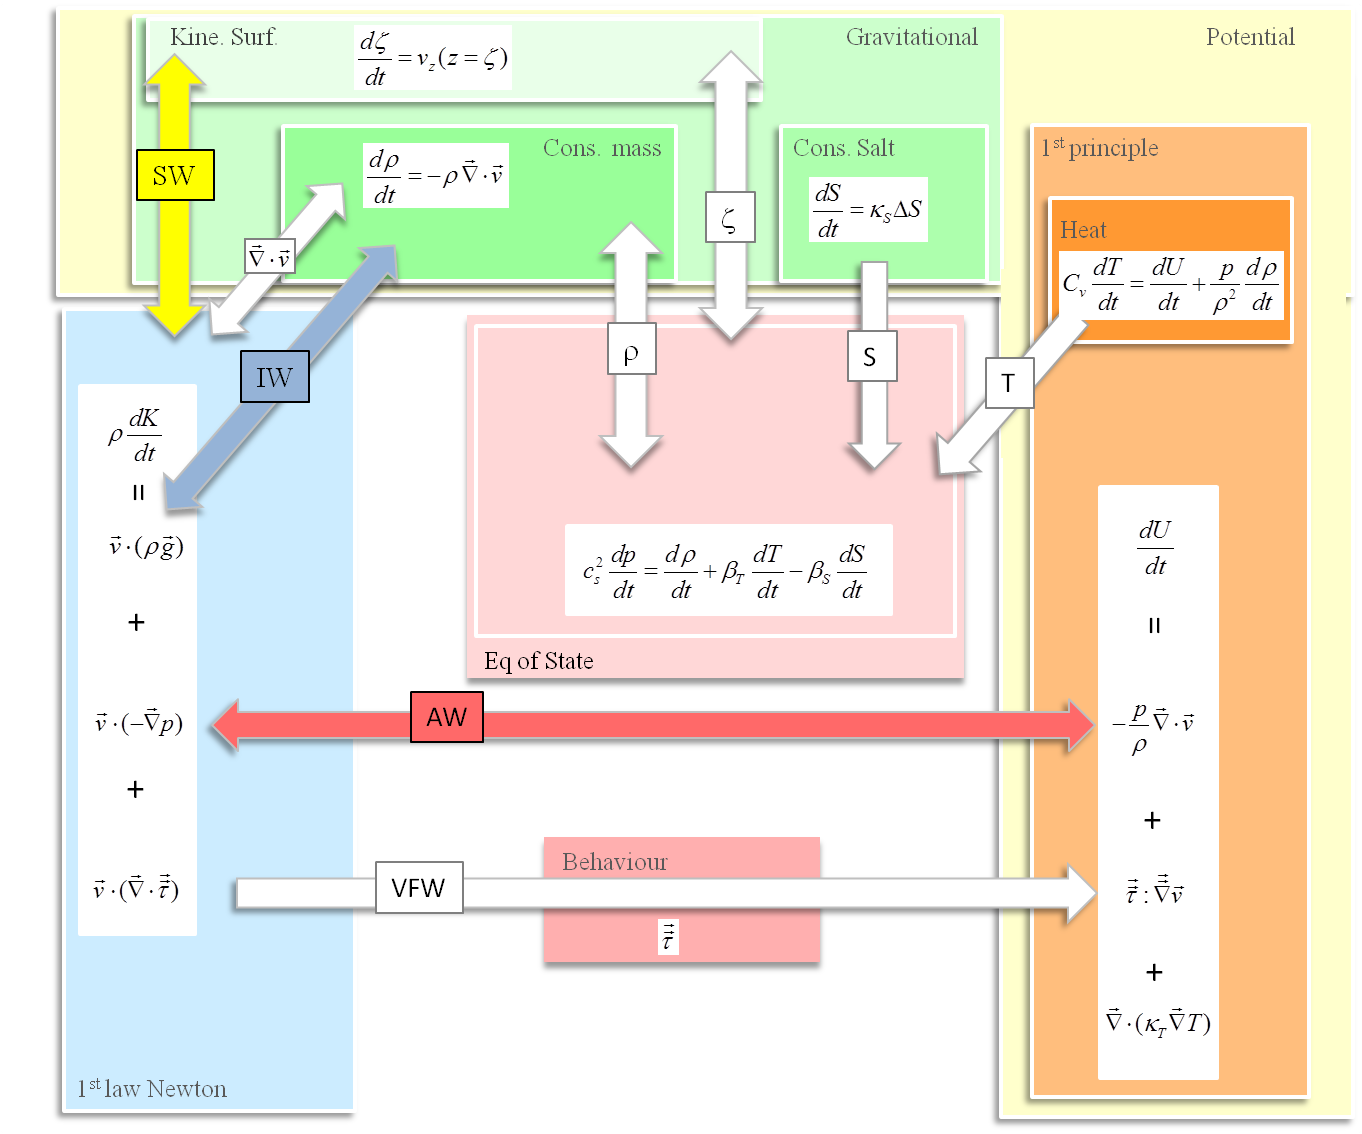
\includegraphics[width=1\linewidth]{FIGURES/MapA.png}
		\caption{}
	\end{subfigure}
	~
	\centering
	\begin{subfigure}{0.49\linewidth}
		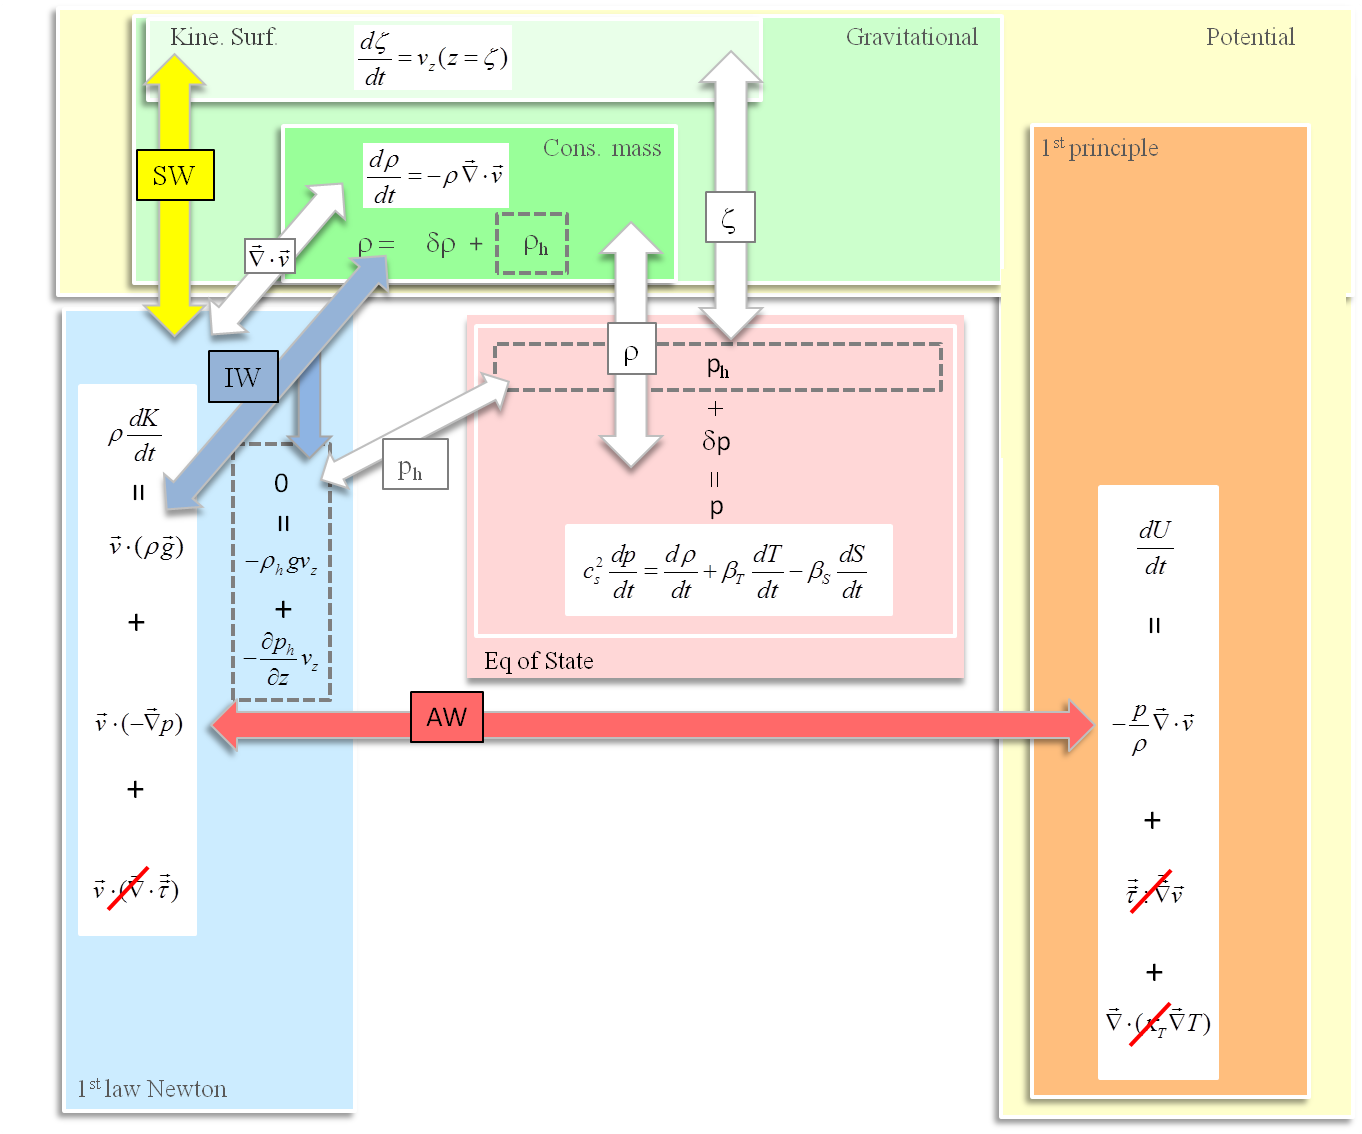
\includegraphics[width=1\linewidth]{FIGURES/MapD.png}
		\caption{}
	\end{subfigure}
	
\caption{ \textit{schematic maps of model equations for a closed ocean.  \textbf{(a)} General model. \textbf{(b)} Simplified P-$\rho$ inviscid model.  \textbf{Boxes}:  EOS (light pink), Comportment (dark pink) kinetic energy (light blue), potential energy (yellow) with gravitational potential (green) and internal energy (orange).  \textbf{White arrows}: Viscous Force Work rate (VFW) and exchanged variables (T, S, $\rho$, $v_z$, $\zeta$ ...).  \textbf{Color arrows}: acoustic waves (AW, red), internal waves (IW, dark blue), surface waves (SW, yellow).}}
	\label{ModelMap}
\end{figure}

To introduce and evaluate simplifications, Figure \ref{ModelMap} shows a schematic map of the complete ocean model. Each colour box is related to a particular compartment of energy: kinetic energy is in light-blue, potential energy is in yellow and, in this later box, internal energy is in orange and gravitational potential energy is in green. The light-pink color is used for the EOS and dark-pink is used for the ocean Newtonian comportment law linking constraints and deformations 
$\left(\vec{\vec{\tau}}=\mu(\vec{\vec{\nabla}}\vec{v}+\vec{\vec{\nabla}}\vec{v}^{\ T})
 +\mu_2(\vec{\nabla}\cdot\vec{v})\ \vec{\vec{I}}\ \right) $. 
White and gray arrows either show transfers between the energy compartments or indicate quantities (variables) exchanged between these compartments. Color arrows indicate energy transfers associated to acoustic, internal and surface waves.
The free-surface anomaly is also indicated in the upper part of the maps, showing that the surface kinematic relation (the prognostic equation for surface anomaly) links the kinematic and potential energy compartments.\\
What the first map (Figures \oldref{ModelMap}.a) confirms at first glance is that the EOS plays a central role in the energy transfers and thus in the dynamics of the ocean and in the propagation mechanisms of ocean waves. 
Ocean waves appears in such a map as oscillatory transfers of energy between two energy compartments (color arrows). 
Acoustic waves induces such transfers between the kinematic and internal wave compartments (AW red arrow). \textit{"The (...) acoustic wave is, actually, the only type of wave out of all these that the fluid's mechanical properties can support in the absence of an external force field (magnetic, gravitational or Coriolis), a pre-existing flow, or a two-component system"}, \cite{lighthill_1967}. Acoustic waves are indeed associated to a balance between ocean compressibility (the restoring mechanism) and inertia. The compressible EOS describes the way the ocean fluid particle "resists" to volume change and the divergence of the velocity links the evolution of momentum (inertia) to the conservation of mass (expressed for density) as respectively indicated by white arrows $(\rho)$ and $(\vec{\nabla}\cdot\vec{v})$.\\
Surface waves (SW yellow arrow) and internal waves (IW blue arrow) are both associated to a transfer of energy between the kinematic and gravitational potential energy compartments. These waves are this time associated to a balance between gravity (the restoring force in the vertical momentum equation) and inertia. They differ by the way mass anomalies evolve. For internal waves, the conservation of mass and the EOS provides this evolution. For surface waves, these two equations provides the evolution of mass in the water column but the surface kinematic relation is required to prognosticate the free-surface anomaly $(\zeta)$. This later anomaly is then involved in the localisation of the boundary condition for pressure.\\
If the objective is to model both acoustic and gravity waves, the associated energy transfers between compartments must thus be modelled with sufficient precision to allow propagation and to avoid energy leaking. Figure \oldref{ModelMap}.d shows a simpler, inviscid model of both acoustic and gravity wave propagations with a limited number of variables. This is the map of the model that shall be used in the present study. Temperature and salinity are not prognostic variables any more. Density includes temperature and salinity contributions but the specific contributions of these variables are modelled implicitly. The exchanges associated to acoustic, internal and surface waves remain. Pressure and density are further decomposed into a reference hydrostatic component $(p_h)$ and $(\rho_h)$ and a non-hydrostatic anomaly (a non-hydrostatic increment) $(\delta p)$ and $(\delta\rho)$ (gray dashed boxes). The hydrostatic decomposition is nothing but a balance between gravity and pressure forces and as such it is associated to low frequency description of the IW energy transfer. It an be viewed as a low-pass filter applied to the vertical momentum equation. It provides a short-cut for a slowly evolving component of internal waves and the non-hydrostatic increment is then the high-frequency increment involving both horizontal and vertical inertia.\\

\subsection{Pressure and density decompositions and EOS simplification}
\label{SubSectionPRHO}

Waves are defined as small disturbances to a motionless, thermodynamic equilibrium state and both pressure and density are decomposed into an equilibrium component and a small increment. Furthermore, the impact of the atmospheric pressure $(p_{atm})$ is neglected to a first approximation, it can indeed take an active part in the generation of the waves, but only play a minor role during the propagation itself. 

Two usual decompositions are thus now formalized for pressure \ref{decompoP_f} and density \ref{decompor_f}:
\begin{subequations}
  \begin{alignat}{2}
  % Pressure decomposition
  \displaystyle 
  \label{decompoP_f}
  \nonumber&p(\mathbf{x},t) &&= 
  \underbrace{\underbrace{p_{atm}
  (\mathbf{x_{\scriptscriptstyle H}},t)}_{\approx0}
  +g\int_z^{\zeta}{\rho_{h}{(\mathbf{x},t)}\ dz}}_{p_h(\mathbf{x},t)}
  +\delta p(\mathbf{x},t)\\[3mm]
  & &&= \underbrace{
  \underbrace{g\int_z^{\zeta}{\displaystyle \hat{\rho}_h(z)}dz}_{\hat{p}_h(z)}
  +\underbrace{g\int_z^{\zeta}{\left(\rho_{h}{(\mathbf{x},t)}-\hat{\rho}_h(z)\right)\ dz}}
  _{p_h'(\mathbf{x},t)}}_{p_h(\mathbf{x},t)}
  +\delta p(\mathbf{x},t)\\[3mm]
  \label{decompor_f}  
  % Density decomposition
  \nonumber&\rho(\mathbf{x},t) &&=\underbrace{\hat{\rho}_{TS}(z)+\rho_{TS}'(\mathbf{x},t)}_{\rho_{TS}(\mathbf{x},t)=\rho(T,S,p=0)}
  +\underbrace{\frac{1}{c_s^{2}}\left(\hat{p}_h(z)+p_h'(\mathbf{x},t)+\delta p(\mathbf{x},t)\right)}_{(\partial \rho / \partial p)_\eta p(\mathbf{x},t)} 
  +\mathrm{O}(p^2)\\[3mm]
  & &&\approx\underbrace{\underbrace{\hat{\rho}_{TS}(z)
  +\frac{\hat{p}_h(z)}{c_s^{2}}}
  _{\hat{\rho}_h(z)}
  +\underbrace{\rho_{TS}'(\mathbf{x},t)
  +\frac{ p_h'(\mathbf{x},t) }{c_s^{2}}}_{\rho_h'(\mathbf{x},t)}  }
  _{\rho_h(\mathbf{x},t)}
  +\frac{\delta p(\mathbf{x},t)}{c_s^{2}}
  \end{alignat}
\end{subequations}
\noindent with $\partial \rho / \partial p = c_s^2$ at constant entropy, $\partial \hat{p}_h /\partial z = -\hat{\rho}_h(z) g$, $\partial p_h' /\partial z = -\rho_h'(z) g$ and $N^2(z)=-g/\hat{\rho}(z)\ \partial \hat{\rho}(z)/\partial z$. A vertical length scale $D(z)$ can be defined by $D(z)=g/N^2(z)$.\\

The first decomposition $(p=p_h+\delta p)$ is based on an hydrostatic component $(p_h)$ and a non-hydrostatic pressure increment $(\delta p)$ is defined. This decomposition has already been introduced in model map (\oldref{ModelMap}.b); it is based on a split of the pressure field between a slowly varying component supposedly in hydrostatic equilibrium and quicly varying non-hydrostatic component. Density can in turn be decomposed in a similar way with $\rho_h$ the hydrostatic component and $\delta \rho=\delta p/c_s^2$ the non-hydrostatic increment. The hydrostatic component of density can be further decomposed in a depth-averaged value $(\hat{\rho}_h(z))$ and a depth-dependant increment $(\rho'_h)$ leading to a similar decomposition for the hydrostatic component of pressure between a surface induced, barotropic component $(\hat{p}_h)$ and a baroclinic increment $(p'_h)$ .\\
The second decomposition focuses on compressibility: it can be viewed as a first order approximation of the EOS with respect to total pressure $(p)$. This Taylor development is carried out in the vicinity of pressure
 It is this time formulated for density.
 $(\rho=\rho_{TS}+p/c_s^2)$ is based on a first order decomposition with respect to total pressure $(p)$. The component $\rho_{TS}$ is a function of temperature and salinity and $p/c_s^2$ is the first-order compressibility increment due to total pressure. \\ 
 Figure (\oldref{ModelMap}.b) indicates that basic transfers between energy compartments associated to acoustic, internal and surface waves are possible under the assumption that temperature and salinity induced processes are implicitely model through the evolution of the density field.
The EOS \ref{NS_e} can be simplified and written in differential form:
\begin{subequations}
\begin{alignat}{2}
	\displaystyle 
	 \frac{\textrm{d}\rho}{\textrm{dt}}=
	\frac{1}{c_s^2}  \frac{\textrm{d} p}{\textrm{dt}}
	\label{EqEOSd}
\end{alignat}
\end{subequations}
Without loss of generality, the present study can now be restricted to the (O, x, z) vertical plan to simplify notations. Equation \ref{EqEOSd} can then be expanded to:
\begin{subequations}
\begin{alignat}{2}
	\label{EqEOS1}
	\displaystyle 
	 \frac{\partial\rho}{\partial t} 
	 +u \frac{\partial \rho}{\partial x}
	 +w \frac{\partial \rho}{\partial z}=
	 \frac{\partial  \rho_{TS}}{\partial t} 
	 +u \frac{\partial  \rho_{TS}}{\partial x}
	 +w \frac{\partial  \rho_{TS}}{\partial z}
	 +\frac{1}{c_s^2}\left(\frac{\partial p}{\partial t} 
	 +u \frac{\partial p}{\partial x}
	 +w \frac{\partial p}{\partial z}\right)
\end{alignat}
\end{subequations}
%At first order (XXX), the equation of state simplifies to:
%\begin{subequations}
%\begin{alignat}{2}
%	\label{EqEOS1}
%	\displaystyle 
%	 \frac{\partial\rho}{\partial t} 
%	 +w \frac{\partial \rho}{\partial z}=
%	 +\frac{1}{c_s^2}\left(\frac{\partial p}{\partial t} 
%	 +w \frac{\partial p}{\partial z}\right)
%\end{alignat}
%\end{subequations}
A Taylor expansion of model equations can now be carried out in the vicinity of the reference profiles $(\hat{p}_h(z),\ \hat{\rho}_h(z))$. Small amplitude wave-induced increments are given by $\delta V\ =\ (p'_h+\delta p,\ \rho'_h+\delta p/c_s^2,\ u ,\ w)$.
At first order in $\delta V$, conservation of mass and vertical advection of pressure and density can be rewritten:
\begin{equation}
	\displaystyle
	\frac{\partial \rho}{\partial t}=-\left(
    	\frac{\partial  \hat{\rho}_{h}u}{\partial x}
	 + \frac{\partial  \hat{\rho}_{h}w}{\partial z}\right) 
	 +\mathrm{O}(\delta V^2),
\end{equation}
\begin{equation}
	\displaystyle
 	w\frac{\partial p}{\partial z}=w\frac{\partial \hat{p}_h}{\partial z}
	 +\mathrm{O}(\delta V^2)
 =-\hat{\rho}_h gw	
	 +\mathrm{O}(\delta V^2)
\end{equation}
and
\begin{subequations}
  \begin{alignat}{2}
	\displaystyle
	& c_s^2w\frac{\partial \rho}{\partial z }
	&&=c_s^2w\frac{\partial \hat{\rho}_{h}}{\partial z }+\mathrm{O}(\delta V^2)
	=-c_s^2 \frac{N^2}{g} w\ \hat{\rho}_{h}
	 +\mathrm{O}(\delta V^2)
	 = -\frac{c_s^2}{D(z)} w\ \hat{\rho}_{h} 
	 +\mathrm{O}(\delta V^2)
 \end{alignat}
\end{subequations}

Substituting these relations in equation \ref{EqEOS1} and isolating pressure variation:
\begin{subequations}
  \begin{alignat}{2}
 \nonumber& \frac{\partial p}{\partial t} &&=
 -c_s^{2}\left(\frac{\partial \hat{\rho}_h u}{\partial x}
 +\frac{\partial \hat{\rho}_h w}{\partial z}\right)
 +\left(g-\frac{c_s^2}{D(z)}\right)\hat{\rho}_h w+\mathrm{O}(\delta V^2)
  \end{alignat}
\end{subequations}
other forms in terms of Buoyancy frequency are:
\begin{equation}
 \frac{\partial p}{\partial t} =
 -c_s^{2}\left(\frac{\partial \hat{\rho}_h u}{\partial x}
 +\frac{\partial \hat{\rho}_h w}{\partial z}\right)
 +\underbrace{\left(g-\frac{c_s^2 N^2}{g}\right)}_{-c_s^2 N_c^2/g}
 \hat{\rho}_h w+\mathrm{O}(\delta V^2)
 \label{Eq_EOS1}
\end{equation}
where $N_c=\sqrt{N^2-g^2/c_s^2}$ is the Brunt-Väisälä frequency for a compressible ocean (\cite{gill_1982}, p169). The free-surface variations are introduced through the surface boundary condition for pressure:
\[
 p(z=0) = \hat{\rho}_h(0) g \zeta+\mathrm{O}(\delta V^2)
\]
 and the kinematic boundary condition can be written for pressure:
\[
 \frac{\rm{d}p}{\rm{dt}}(z=0)= g \hat{\rho}_h(0) w(z=0)+\mathrm{O}(\delta V^2)
\]

\bigbreak
\subsection{Linear, inviscid wave model}
\label{SubSectionLinModel}

Based on the pressure and density decompositions proposed in subsection \ref{SubSectionPRHO}, the simpler, inviscid, linear, rotation-less $(p-\rho)$ model mapped on figure (\oldref{ModelMap}.b) can be used to model acoustic, internal and surface waves. At first order in wave-induced increments $\delta V$, the conservations of horizontal and vertical momentums and mass and the EOS are written as:
\begin{subequations}
  \begin{alignat}{2}
    \displaystyle
    \label{WM_a}
    % NS in x-direction:
     &\frac{\partial\hat{\rho}_h u}{\partial t} &&  \approx 
     -\frac{\partial p}{\partial x}\\[3mm]    
    \label{WM_b}
    % NS in z-direction:
    &\frac{\partial \hat{\rho}_h w}{\partial t} && \approx 
    -\frac{\partial p}{\partial z}-\rho g \\[3mm]
    \label{WM_c}
    %Continuity equation:
    &\frac{\partial \rho}{\partial t} && \approx  - (\frac{\partial \hat{\rho}_h u}{\partial x}+\frac{\partial \hat{\rho}_h w}{\partial z}) \\
    \label{WM_d}
    % State equation  or Pressure equation:
    & \frac{\partial p}{\partial t} &&\approx
 -c_s^{2}\big(\frac{\partial \hat{\rho}_h u}{\partial x}
 +\frac{\partial \hat{\rho}_h w}{\partial z}\big)
 -\overbrace{\left(\frac{c_s^2}{D(z)}-g\right)}^{c_s^2 N_c^2/g}\hat{\rho}_hw
  \end{alignat}
\end{subequations}
with the bottom and surface relations:
\begin{subequations}
  \begin{alignat}{2}
    \displaystyle
    \label{WM_bc_a}
  &w(z=-H) && =0 \\[3mm]
    \label{WM_bc_b}
  &\frac{\partial p}{\partial t}(z=0) && \approx \hat{\rho}_h g w(z=0)
  \end{alignat}
\end{subequations}

The terms associated to the color arrows plotted on figure (\oldref{ModelMap}.d) can be identified in the above equations:
\begin{itemize}
	\item acoustic waves: compressibility is represented by the first term on the right-hand-side of EOS \ref{WM_d} and the internal mode compartment is not explicitly modelled.
	\item surface waves: the gravity force $(-\rho g)$ in Eq \ref{WM_b} is involved in energy transfers with the gravitational potential compartment through the surface kinematic relation \ref{WM_bc_b}.
	\item internal waves: the gravity force $(-\rho g)$ in Eq \ref{WM_b} is involved in energy transfers with the gravitational potential compartment, mass balance is insured by Eq \ref{WM_c}. A first-order approximation (in $\delta V$) of advection is given by $(-\frac{c_s^2 N_c^2}{g} \hat{\rho}_h w)$ in Eq \ref{WM_d}, this term gathers vertical advection of isobaric (last part of over-brace development) and isopycnal (first part) surfaces.
\end{itemize}
The surface kinematic condition \ref{WM_bc_b} is specified here in an Eulerian form but at $z=0$ which is a first-order approximation of its true location $(z=\zeta)$. This approach differs from the Lagrangian approach proposed by Dukowicz (Dukowicz, 2015). Even if we can agree with the fact that the motion of the free-surface of the ocean is fundamentally Lagrangian, a somehow-simpler Eulerian approach remains possible in non-Boussinesq context and, in the present case, both approaches lead to the same dispersion relations.


%\section{General polarization and dispersion for acoustic-gravity waves}
%\label{SectionDisp}

\subsection{General propagation equation and polarization}

\textit{Form of the wave solutions:}\\
Dispersion relations can be derived by postulating and specifying the form of the waves. Horizontally-propagating surface waves, wave-modes propagating in the ocean wave-guide, internal wave-rays and acoustic waves all satisfy the following "polarization" relations:
\label{SubSectionPropag}
\begin{subequations}
  \begin{alignat}{2}
  \displaystyle
  \left(
  \begin{array}{c}
    \hat{\rho}_h u\\
    \hat{\rho}_h w\\
    \rho\\
    p
  \end{array}
  \right)
  =
  \left(
  \begin{array}{c}
    \widetilde{U}(z)\\
    \widetilde{W}(z)\\
    \widetilde{\rho}(z)\\
    \widetilde{p}(z)
  \end{array}
  \right)
  e^{i(k_xx-\Omega t)}
\end{alignat}
\end{subequations}
where $k_x$ and $\Omega$ are respectively the horizontal wave-number and the pulsation of the wave. \\

\textit{Inner dispersion relation:}\\
These relations can be substituted in propagation model \ref{WM_a} to \ref{WM_d}.  After lengthy developments, an ordinary differential equation can be obtained for $ \widetilde{W}(z)$ :
\begin{equation}
  \displaystyle
  \widetilde{W}''(z)+\frac{1}{D(z)}\widetilde{W}'(z)
  +
  \left(
  k_x^2\frac{N_c^2-\Omega^2}{\Omega^2}+\frac{\Omega^2}{c_s^2}
  -\frac{D'(z)}{D^2(z)}
  \right)
  \widetilde{W}(z)=0
  \label{eqwfirst}
\end{equation}
and to remove first order term and simplify future development, the following change of variable can be made:
\begin{equation}
  \displaystyle
  \widetilde{W}(z)=e^{\int_{z}^0{ \frac{\rm{d} z_1}{2D(z_1)} } }F(z)
  \label{CVF}
\end{equation}
where $D(z)$ is the scale-depth i.e. the vertical scale-length associated to the stratification. It gives an idea of the vertical distance over which a $1\ kg/m^{-3}$ density change can be observed.
The unknown function $F(z)$ satisfies:
\begin{equation}
  \displaystyle
  F''(z)
  +\left(
  k_x^2\frac{N_c^2-\Omega^2}{\Omega^2}
  +
  \frac{\Omega^2}{c_s^2}-\frac{1+2D'(z)}{4D(z)^2}
  \right)
  F(z)=0
  \label{eqF}
\end{equation}
The unknown function $F(z)$ differs from the vertical momentum $W(z)$ by the attenuation factor $e^{\int_{z}^0{ \frac{\rm{d} z_1}{2D(z_1)} } }$. This factor reduces the vertical extent of the wave anomalies based on the length scale $D(z)$. The stronger the stratification, the larger $D(z)$ and the shorter this vertical extent.\\

\textit{Boundary dispersion relation:}\\
The polarization relations must also be substituted in the surface boundary condition \ref{WM_bc_b} leading to:
\begin{equation}
  \displaystyle
  -i\Omega P(0)=g \widetilde{W}(0)
\end{equation}
or
\begin{equation}
  \displaystyle
  \widetilde{W}'(0)+\left(
  \frac{1}{D(0)}-\frac{gk_x^2}{\Omega^2}
  \right)\widetilde{W}(0)=0
\end{equation}
In term of the unknown function $F(z)$, this relation can be written as:
\begin{equation}
  \displaystyle
  F'(0)+\left(
  \frac{1}{2D(0)}-\frac{gk_x^2}{\Omega^2}
  \right)F(0)=0
  \label{eqFbc}
\end{equation}
The bottom boundary condition \ref{WM_bc_a} simply leads to:
\begin{equation}
  \displaystyle
  F(-H)=0
  \label{eqFbc2}
\end{equation}

\textit{Constant Brunt-Väisälä pulsation:}\\
In the following sections, $D(z)\approx D_0$ (or equivalently $N^2\approx N_0^2$) should be quasi-constant and relation \ref{CVF} can be rewritten:
\begin{equation}
  \displaystyle
  \widetilde{W}(z)=e^{-\frac{z}{2D_0}}F(z)
  \label{CVF2}
\end{equation}
showing that the larger the stratification (i.e. the larger $D_0$), the smaller the vertical extent of the wave. The stratification classically prevent vertical propagation.\\
The general expression of the vertical velocity perturbation profile for a constant scale height $D_0$ is
\begin{equation}
  \displaystyle
  w(x,z,t)=\frac{1}{\hat{\rho}_h(z)}\widetilde{W}(z)e^{i(k_x-\Omega t)},
\end{equation}
with $\hat{\rho}_h(z)=\hat{\rho}_h(0)e^{-z/D_0}$ and then
\begin{equation}
  \displaystyle
  \begin{array}{rcl}
  	\widetilde{W}(z)&=&e^{-z/(2D_0)}F(z)\\[4mm]
    \widetilde{U}(z)&=&\displaystyle  -ik_x\frac{(c_s^2-gD_0)\widetilde{W}(z)+c_s^2D_0\widetilde{W}'(z)}{D_0(\Omega^2-c_s^2k_x^2)}\\[4mm]
    \widetilde{\rho}(z)&=&\displaystyle -i\frac{k_x^2(c_s^2-gD_0)\widetilde{W}(z)+\Omega^2D_0\widetilde{W}'(z)}{D_0\Omega(\Omega^2-c_s^2k_x^2)}\\[4mm]
    \widetilde{p}(z)&=&\displaystyle -i\Omega\frac{(c_s^2-gD_0)\widetilde{W}(z)+c_s^2D_0\widetilde{W}'(z)}{D_0(\Omega^2-c_s^2k_x^2)}
\end{array}
\end{equation}

\subsection{Inner and boundary dispersion relations}
 \label{SubSectionDisp}
 
 \subsubsection{Dimensional dispersion relations}
When the Brunt-V\"ais\"al\"a frequency $N$ is constant, the scale-depth is constant $D(z)=D_0$ and the solution is obtained by solving the system:
\begin{subequations}
	\label{EqDimF}
	\begin{alignat}{2}	
    \displaystyle
	\label{EqDimFa}
    F''(z)
    +
   \overbrace{ \left(k_x^2\frac{N_c^2-\Omega^2}{\Omega^2}+\frac{\Omega^2}{c_s^2}-\frac{1}{4D_0^2}\right)}^{\equiv k_z^2}
    F(z)=0\\[4mm]
	\label{EqDimFb}
    \displaystyle
    F'(0)+\left(
    \frac{1}{2D_0}-\frac{gk_x^2}{\Omega^2}
    \right)F(0)=0\\[4mm]
	\label{EqDimFc}
    \displaystyle
    F(-H)=0
  \end{alignat}
\end{subequations}
The square of the vertical wave-number $k_z$ is defined in \ref{EqDimFa} and is a function of $k_x$ and $\Omega$, it can be positive or negative which only guarantees that $k_z \in \mathbb{R}$ or $k_z \in i\mathbb{R}$. The unknown function $F(z)$ is then a linear combination of $e^{\pm k_z z}$. This consequently leads to a first dispersion relation in dimensional form:
\begin{equation}
  \label{EqDispRefInner}
  \displaystyle
   k_x^2\left(1-\frac{N_c^2}{\Omega^2}\right)+k_z^2
   -\frac{\Omega^2}{c_s^2}+\frac{1}{4D_0^2}=0
\end{equation}
This relation does not take into account the boundary conditions at the surface nor at the bottom and consequently only deals with the propagation of waves in the inner ocean. It shall now be referred to as the \textit{inner dispersion relation}.

The general solution that satisfies the bottom boundary condition \ref{EqDimFc} is
\begin{equation}
	\label{EqDispRef}
  	\displaystyle
  	F(z)=\sin\left(k_z(H+z)\right).
\end{equation}
%which leads to
%\begin{equation}
%  \displaystyle
%  w(x,z,t)=\hat{\rho}_h(0)e^{z/(2D_0)}\sin(k_z(H+z)).
%\end{equation}
The surface boundary condition \ref{EqDimFb} leads then to the dispersion relation:
\begin{equation}
	\label{EqDispRefs}
     \Omega^2 =\frac{gk_x^2\ tan(Hk_z)}{k_z +\frac{ tan(Hk_z)}{2 D_0 }}
    =\frac{gk_x^2 }{\frac{1}{ 2 D_0} + k_z cotan(Hk_z)}
\end{equation}
A wave propagating in a "bounded ocean" must satisfy both the \textit{inner} and \textit{boundary} (dimensional) dispersion relation \ref{EqDispRefInner} and \ref{EqDispRefs}.

\subsubsection{Dimensionless dispersion relations}
Two parameters can now be defined to obtain dimension-less dispersion relations:
\begin{equation}
     \epsilon_i^2 =  \frac{N_c^2 H}{g} 
    ,\ \epsilon_a^2 = \frac{g H}{c_s^2} 
\end{equation}
$\epsilon_i$ is thus a small gravity parameter defined as the ratio of the order of magnitude of internal wave mode one $(N_c H)$ to the velocity of long surface waves $(\sqrt{gH})$, see section \ref{SectionGraphic}.
$\epsilon_a$ is a small acoustic parameter defined as the ratio of the velocity of long surface waves $(\sqrt{gH})$ to sound waves $c_s$. Note that $\epsilon_i$ is defined with the compressible Brunt-Väisälä frequency $N_c$, i.e. the Brunt-Väisälä frequency $N$ modified by compressibility effects (this notation has been introduced in Eq \ref{Eq_EOS1}). Three dimensionless variables are further defined:
\begin{equation}
    \left( \omega = \Omega \sqrt{\frac{H}{g}}
    ,\ \delta_x = k_x H
    ,\ \delta_z = k_z H \right)
\end{equation}
The constant scale-depth can be rewritten: $D_0=H/(\epsilon_i^2+\epsilon_a^2)$.  Note that this scale-depth does not include any compressibility-induced correction and, as a consequence, it is a function of both small parameters $\epsilon_i$ and $\epsilon_a$. As a consequence the stratification scale-depth ratio $H/D_0=\epsilon_i^2+\epsilon_a^2$ give an idea of the relative strength of the ocean stratification.\\
A set of two dimensionless dispersion relations are thus eventually obtained:
\begin{subequations}
	\label{EqFullDisper}
	\begin{alignat}{2}	
		\label{EqFullDispera}
 		& \delta_x^2+\delta_z^2 &&=\epsilon_i^2\frac{\delta_x^2}
 			{\omega^2}+\epsilon_a^2\omega^2-\frac{(\epsilon_a^2+\epsilon_i^2)^2}{4}\\[3mm]
		\label{EqFullDisperb}
		& \omega^2 &&=\frac{\delta_x^2\ tan(\delta_z)}
		{\delta_z+\frac{\epsilon_a^2+\epsilon_i^2}			{2}tan(\delta_z)}
		%=\frac{\delta_x^2}{\frac{\epsilon_a^2+\epsilon_i^2}{2}
		%+\delta_z cotan(\delta_z)}
	\end{alignat}
\end{subequations}
The first relation is the dispersion relation for the inner-ocean. It derives from equations \ref{WM_a} to \ref{WM_d}. The second one (hereafter the \textit{boundary dispersion relation}) is the dispersion relation deriving from the surface and bottom boundary conditions \ref{WM_bc_b}.
In a free-surface ocean, wave solutions must satisfy both relations. This means that only one of the parameters among the pulsation $\omega$ and the horizontal and vertical wave-numbers ($\delta_x$ and $\delta_z$) can be settled by forcing, the remaining two adjusting so that the wave satisfies the two dispersion relations. For short vertical-wave-number and far for the bottom and surface boundaries, wave solutions can satisfied only the inner dispersion relation and be dynamically consistent. Purely acoustic waves or pure internal-gravity wave-rays are for instance known to propagate in the inner ocean as in an unbounded ocean.\\
%The system of dispersion equations \ref{EqFullDisper} is a system of 2 dispersion equations with 3 unknowns $(\omega,\ \delta_x,\ \delta_z)$ leaving one degree of freedom that is left for any kind of forcing initiating at least one of the possible wave solutions. 
%One way to investigate these wave solution solutions is to consider that forcing is thus responsible for the value taken by one of the variable (hereafter either $\omega$ or $\delta_x$ will alternatively be this \textit{forced} variable) before expressing the remaining two variables as functions of the \textit{forced} variable.\\

%To better understand their impact in the set of physical equations presented in subsection \ref{SubSectionLinModel}, a few "often-neglected" terms  are now temporally dropped and the dispersion relations are re-derived. When the gravity force or, for a similar result, the zeroth-order vertical term in the pressure equation are neglected in respectively the horizontal momentum and the EOS, the dispersion relation simplifies to:
%\begin{subequations}
%	\label{EqFullDisper1}
%	\begin{alignat}{2}	
% 		& \delta_x^2+\delta_z^2 &&=
% 		%\epsilon_i^2\frac{k_x^2}{\omega^2}
% 		\epsilon_a^2\omega^2
% 		-\frac{\epsilon_i^2}{4}\\[3mm]
%		& \omega^2 &&=\frac{\delta_x^2\ tan(\delta_z)}
%		{\delta_z+\frac{\epsilon_a^2+\epsilon_i^2}	{2}tan(\delta_z)}
%	\end{alignat}
%\end{subequations}
%The inner dispersion equation only has one solution in $\omega^2$ :  $\omega^2=\omega_a^2$ whereas the surface dispersion relation remains unchanged. This therefore means that acoustic waves can still propagate but not internal waves. Only part of surface waves can still be modelled. The graphic investigation proposed in section \ref{SectionGraphic} should help us clarify these consequences.\\

Ocean waves can consequently propagate in a $(x,\ z)$ vertical section of a "bounded ocean" if the triplet of wave-properties $(\delta_x,\ \delta_z,\ \omega)$ satisfy the 2 relations \ref{EqFullDispera} and \ref{EqFullDisperb}. This leaves only one degree of freedom to impose forcing (against two for waves propagating in an unbounded ocean). In the rather general context of a stratified and compressible ocean, two parameters $(\epsilon_i,\ \epsilon_a)$ have been identified to render the relative impact of gravity and compressibility in the propagation mechanism. The resulting set of two equations of three variables and two parameters is non-linear and simple general solution cannot be carried out analytically. Much insight can yet be gained in these ocean waves investigating geometrically the inner and boundary surfaces associated to the corresponding dispersion relations. 
Indeed, in $(\delta_x,\  \delta_z,\ \omega)$ phase-space, the inner and boundary dispersion relations are respectively given by two surfaces. When these two surfaces intersect, points lying on the intersection are triplets of wave solutions. The surfaces associated respectively to the inner and boundary relations will respectively be named the \textit{inner and boundary dispersion surfaces}.

Several difficulties can be anticipated. Firstly, one already noted in subsection \ref{SubSectionDisp} that the inner dispersion relations were fourth-order relations in $(\delta_x,\ \delta_z,\ \omega)$, a consequence being that the corresponding surfaces are quartics and shall only be associated locally to simpler, well-known quadric surfaces (i.e. under further assumptions that will have to be clearly stated). Intersections and roots can indeed be simply derived analytically in this latter case. A consequence is that several local approximations will have be proposed, each corresponding to one type of waves associated to one set of parameters. A second major difficulty to carry out some analytical investigation is that the boundary dispersion relation is a transcendental relation and the intersections with the inner dispersion surface, when they exist, can not be easily derived and further investigation  requires additional assumptions.\\

%%%%%%%%%%%%%%%%%%%%%%%%%%%%%%%%%%%%%%%%%%%%%%%%%%%%%%%%%%%%%%%%%%%%%%%%%%%
\newpage
%%%%%%%%%%%%%%%%%%%%%%%%%%%%%%%%%%%%%%%%%%%%%%%%%%%%%%%%%%%%%%%%%%%%%%%%%%%
\section{Inner dispersion relation \& waves in an unbounded ocean}
\label{SectionInner}
%%%%%%%%%%%%%%%%%%%%%%%%%%%%%%%%%%%%%%%%%%%%%%%%%%%%%%%%%%%%%%%%%%%%%%%%%%%

The inner dispersion relation \ref{EqFullDispera} must be satisfied by any type of ocean waves whether the ocean can or cannot be locally considered as an unbounded medium (far from its surface and bottom). We shall show in the present section that (i) in $(\delta_x,\  \delta_z,\ \omega)$ phase-space, the inner dispersion relation leads to a three-branch dispersion surface, (ii) the acoustic and stratification factorization functions $\omega_a(\delta_x,\ \delta_z)$ and $\omega_i(\delta_x,\ \delta_z)$ can be good approximations of the branches, (iii) the upper and lower branches of the inner dispersion surface (for respectively large and low pulsations) correspond to acoustic waves and internal rays propagating in an unbounded ocean and (iv) the bounded central branch of the inner dispersion surface corresponds to vertically vanishing waves

%To further investigate the inner dispersion relation \ref{EqFullDispera}, the evolution of the vertical wave-number $\delta_z$ as a function of the horizontal wave-number $\delta_x$ and of the pulsation $\omega$ is now further investigated. Note that the case of long waves will be considered separately in the following sections so that $\delta_x$ and $\delta_z$ do not need to be simultaneously small to start with.

%\subsection{Branches of the inner dispersion relation: compressibility \& stratification.}
%\subsection{Branches of the inner dispersion relation}
\subsection{Factorizing functions and roots of the inner dispersion relation}
\label{SubSectionFactoDisp}

All terms in the inner dispersion relation (whether $\delta_z$ is real or pure imaginary) are quadratic in $(\delta_x,\ \delta_z,\ \omega)$ expect the first term of the right-hand-side $(\epsilon_i^2 \delta_x^2/\omega^2)$ which is quadratic in $\delta_x$ and inversely proportional to the square of the pulsation. It is related to the ocean stratification and brings in internal gravity waves. A further investigation shows that this term is in fact associated to vertical advection through last term of the state equation \ref{WM_d}. After multiplication by $\omega^2$ to avoid a singularity for $\omega = 0$ (see Eq. \ref{eqomegaparam2} bellow), the inner dispersion relation for stratified ocean is fourth order in $(\delta_x,\ \delta_z,\ \omega)$, increasing somehow the analytical burden. The boundary dispersion relations \ref{EqFullDisperb} includes a transcendental function ($tan(delta_z)$ with $\delta_z\in\mathbb{C}$).

\subsubsection{Acoustic and stratification factorizing functions $(\omega_a,\ \omega_i)$}
\label{subsubsectionFacto}
To gain insight in the physics of the wave solutions, the inner dispersion relation \ref{EqFullDispera} can be written as:
\begin{equation}
\omega^2
	\left(
	\delta_x^2+\delta_z^2
	+\frac{(\epsilon_a^2+\epsilon_i^2)^2}{4}
	-\epsilon_a^2\omega^2
	\right)
	=\epsilon_i^2 \delta_x^2
	\label{eqomegaparam2}
\end{equation}
which can further be expressed in the simpler form:
\begin{equation}
	\frac{\omega^2}{\omega_a^2}+\frac{\omega_i^2}{\omega^2}=1
	\label{eqlink}
\end{equation}
where $\omega_i$ and $\omega_a$ are functions of the horizontal and vertical wave-numbers and can be defined by
\begin{subequations}
	\label{EqDispSols}
	\begin{alignat}{2}	
	\label{SolAcous}
	& \omega_a^2(\delta_x,\ \delta_z) &&=\frac{1}{\epsilon_a^2}\left(
	\delta_x^2+\delta_z^2
	+\frac{(\epsilon_a^2+\epsilon_i^2)^2}{4}
	\right)\\
	\label{SolGrav}
	&\omega_i^2(\delta_x,\ \delta_z)  &&=
	\frac{\delta_x^2\ \epsilon_i^2}{\delta_x^2+\delta_z^2
	+(\epsilon_a^2+\epsilon_i^2)^2/4}
	\end{alignat}
\end{subequations}
These two functions are not roots of the inner dispersion equation \ref{eqlink} but they can play an important role in the approximation of the roots of this equation and more specifically in their physical interpretation. The factorizing function can indeed be introduced approximating the \textit{inner dispersion} relation \ref{EqFullDispera}:
\begin{itemize}
	\item \textit{If
	$\epsilon_a^2\omega^2 >> \frac{\epsilon_i^2\delta_x^2}{\omega^2}$} (for instance for large pulsations) then \ref{EqFullDispera} simplifies to 
	$\omega^2\approx\omega_a^2$. A compressible, homogeneous (unstratified) ocean satisfies this assumption.
	\item \textit{If now $\epsilon_a^2\omega^2<< \frac{\epsilon_i^2\delta_x^2}{\omega^2}$} (for instance for small pulsations) then \ref{EqFullDispera} simplifies to $\omega^2\approx\omega_i^2$. An incompressible, stratified ocean satisfies this assumption.
\end{itemize}
$\omega_a$ can therefore be interpreted as the factorizing \textit{acoustic function} accounting for the compressibility content of the inner dispersion relation and $\omega_a^2$ is the solution of the \textit{inner} dispersion relation for an homogeneous ocean. $\omega_i$ plays an equivalent role for the ocean stratification: it can be interpreted as the factorizing \textit{stratification function} and $\omega_i^2$ is the solution of the \textit{inner} dispersion relation for an incompressible ocean.\\
Both functions depend on $\epsilon_a^2+\epsilon_i^2 = H/D_0$, the stratification scale-depth ratio with no compressible correction. 
When $\epsilon_a$ tends toward zero (compressibility vanishes), $\omega_a$ approaches infinity and the first term of \ref{eqlink} vanishes for a finite pulsation $\omega$. 
When $\epsilon_i$ tends in turn toward zero (weak stratifications), $\omega_i$ approaches zero and the second term of \ref{eqlink} vanishes if the pulsation $\omega$ remains finite. 

\subsubsection{Roots of the inner dispersion relation $(\omega_\pm)$}
Under the condition $\displaystyle \frac{\omega_i^2}{\omega_a^2}\le \frac{1}{4}$, Eq. \ref{eqlink} has two real roots. Odd powers of the dispersion polynomial equation vanish and the roots can be formulated for the square of the pulsation:
\begin{equation}
	\omega_{\pm}^2
	=\frac{\omega_a^2}{2}
	\left(
	1\pm
	\sqrt{1-4\underbrace{\frac{\omega_i^2}{\omega_a^2}}_{\equiv\ R^2}}
	\right)
\label{solseq}
\end{equation}
The ratio of the acoustic to the stratification functions $R(\delta_x,\ \delta_z)$ plays a central role in the existence and unicity of the roots. The square of this ratio can be expressed as
\begin{equation}
	R^2(\delta_x,\delta_z)=
	\frac{\omega_i^2}{\omega_a^2}=
	\frac{\epsilon_a^2\epsilon_i^2\delta_x^2}
	{\left(\delta_x^2+\delta_z^2
	+\frac{(\epsilon_a^2+\epsilon_i^2)^2}{4}
	\right)^2}
\label{eqratio}
\end{equation}
The condition $\displaystyle R^2(\delta_x,\delta_z)\le \frac{1}{4}$ is required for the dispersion relation \ref{eqomegaparam2} to have a real root. If, on the contrary $\displaystyle R^2(\delta_x,\delta_z) >\frac{1}{4}$, the solution is not an oscillatory wave-solution: its pulsation is complex with both a damped and an amplified solution.\\
For small $\epsilon_i$ and $\epsilon_a$ parameters, these two roots can be compared to the acoustic and stratification functions $\omega_a$ and $\omega_i$:
\begin{subequations}
	\begin{alignat}{2}
	\label{Comp1}
	&\omega_a^2(\delta_x,\ \delta_z)-\omega_{+}^2(\delta_x,\ \delta_z)
	&&=\frac{\epsilon_i^2\delta_x^2}{\delta_x^2+\delta_z^2}
	+\mathrm{O}	(\epsilon_i^p,\epsilon_a^{6-p})\\[3mm]
	\label{Comp2}
	&\omega_{-}^2(\delta_x,\ \delta_z)-\omega_i^2(\delta_x,\ \delta_z)
	&&=\frac{\epsilon_i^4\epsilon_a^2\delta_x^4}{(\delta_x^2+\delta_z^2)^3}
	+\mathrm{O}	(\epsilon_a^q,\epsilon_i^{10-q})
	\end{alignat}	
\end{subequations}
with $(p,\ q)\in\{2,\ 4,\ 6\}^2$. These Taylor developments show that the first root $(\omega_+)$ approaches the \textit{acoustic function} $(\omega_a)$ when the stratification loosen ($\epsilon_i$ tends toward 0). Both $\omega_+$  and $\omega_a$ approach infinity when $\epsilon_a$ tends toward zero (i.e. when compressibility vanishes). The second root $(\omega_-)$ approaches the \textit{stratification function} $(\omega_i)$ when $\epsilon_a$ tends toward zero. $\omega_-$, $\omega_i$ and their difference approach 0 when $\epsilon_a$ tends toward zero (i.e. when stratification weakens). \\
%The second term of \ref{eqlink} vanishes this time if the pulsation $\omega$ remains finite.\\
However $\omega_a$ (receptively $\omega_i$) are good approximations of $\omega_+$ ($\omega_-$) only if $\delta_z\in\mathbb{R}$. Indeed, the sum of the square of the wave-numbers at the denominator of the right-hand-sides of the above relations can be arbitrarily small (even for large $\delta_x$) if $\delta_z\in i \ \mathbb{R}$. In this case, the roots $(\omega_\pm)$ might not be well-approximated by $\omega_a$ and $\omega_i$.\\
To proceed, the dependency of the form and solutions of the inner dispersion relation to the vertical wave-number $\delta_z$ consequently needs to be investigated.

%\subsection{Dispersion relations in $(\delta_x,\ \delta_z,\ \omega)$ phase space}
%\label{SubSectionDispSurfIntro}

%In an unbounded ocean (far from the bottom and of the surface of the ocean), ocean waves only need to satisfy the inner-ocean dispersion relation \ref{EqFullDispera}. Pure internal and acoustic waves are examples of such waves. Many more types of waves can propagate in the ocean but if this assumption is relaxed, waves must satisfy simultaneously the inner and the bottom dispersion relations. These waves can basically be divided in two categories. The first category gathers evanescent waves which do not propagate vertically. Their vertical wave-number is a pure-imaginary complex $(\delta_z\in i\mathbb{R})$. Waves from the second category are usually called "wave modes": they do not propagate vertically either but their vertical wave-number must be "quantified" to satisfy the bottom and surface boundary conditions: it is solution of a discrete eigenvalue problem. As already stated in the introductory review, internal-gravity and acoustic-gravity modes are well-known examples of such modes.\\

%Ocean waves can consequently propagate in a $(x,\ z)$ vertical section of a "bounded ocean" if the triplet of wave-properties $(\delta_x,\ \delta_z,\ \omega)$ satisfy the 2 relations \ref{EqFullDispera} and \ref{EqFullDisperb}. This leaves only one degree of freedom to impose forcing (against two for waves propagating in an unbounded ocean). In the rather general context of a stratified and compressible ocean, two parameters $(\epsilon_i,\ \epsilon_a)$ have been identified to render the relative impact of gravity and compressibility in the propagation mechanism. The resulting set of two equations of three variables and two parameters is non-linear and simple general solution cannot be carried out analytically. Much insight can yet be gained in these ocean waves investigating geometrically the inner and boundary surfaces associated to the corresponding dispersion relations. \\
%Indeed, in $(\delta_x,\  \delta_z,\ \omega)$ phase-space, the inner and boundary dispersion relations are respectively given by two surfaces. When these two surfaces intersect, points lying on the intersection are triplets of wave solutions. The surfaces associated respectively to the inner and boundary relations shall now respectively be named the \textit{inner and boundary dispersion surfaces}.\\

%Several difficulties can be anticipated. Firstly, one already noted in subsection \ref{SubSectionDisp} that the inner dispersion relations were fourth-order relations in $(\delta_x,\ \delta_z,\ \omega)$, a consequence being that the corresponding surfaces are quartics and shall only be associated locally to simpler, well-known quadric surfaces (i.e. under further assumptions that will have to be clearly stated). Intersections and roots can indeed be simply derived analytically in this latter case. A consequence is that several local approximations will have be proposed, each corresponding to one type of waves associated to one set of parameters. A second major difficulty to carry out some analytical investigation is that the boundary dispersion relation is a transcendental relation and the intersections with the inner dispersion surface, when they exist, can not be easily derived and further investigation  requires additional assumptions.\\ 

\subsection{Three regions in $(\delta_x,\ \delta_z,\ \omega)$ phase-space}
\label{SubSectionDeltaz}
\begin{figure}[!h]
	\centering	
	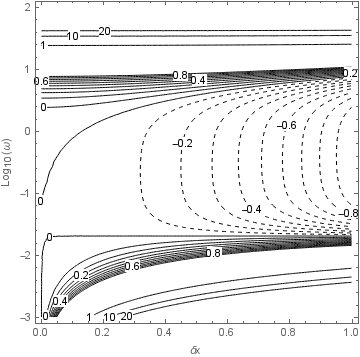
\includegraphics[width=0.5\linewidth]{FIGURES/Contour_dz.png}
	\caption{\textit{contours of $\ \delta_z^2(\delta_x,\ \omega)$}. Plain lines correspond to positive values of $\delta_z^2$ $(\delta_z\in\mathbb{R})$ whereas dashed lines are associated to negative values $(\delta_z\in i\mathbb{R})$.}
	\label{FigContourdz}
\end{figure}
Figure \ref{FigContourdz} shows the variations of the square of the vertical wave-number $(\delta_z^2)$ as a function of $(\delta_x,\ \,\omega)$.  Negative values are encountered for medium-range pulsations $(10^{-0.7}<\omega<10^{0.7})$ and large enough horizontal wave-numbers $(\delta_x \geq 0.1-0.2)$. This region is limited by two regions of positive $\delta_z^2$, one for large pulsations and the other for small pulsation. The transition lines between these regions is given by $\delta_z^2=0$. The description of these two regions begun in Section \ref{subsubsectionFacto} can now be proceeded:
\begin{itemize}
	\item \textit{If $\omega>>1$ and $\epsilon_a>0$ then} $\omega^2\approx\omega_a^2$ and the transition line is given by 
	$\epsilon_a^2\omega^2 \approx
	\delta_x^2
 	+\frac{(\epsilon_a^2+\epsilon_i^2)^2}{4}$. This line is a parabola and the pulsation is not bounded when $\delta_x$ increases. 
 	When $\delta_x$ goes to 0, $\omega$ decreases monotically and reaches its lower bound for $\delta_x=0$: its minimum is given by $\omega_{c,a}=(\epsilon_a^2+\epsilon_i^2)/2\epsilon_a$.
	\item \textit{If $\omega<<1$ and $\epsilon_i>0$ then} $\omega^2\approx\omega_i^2$, the equation of the transition line is $\omega^2\approx\delta_x^2\epsilon_i^2/(\delta_x^2+(\epsilon_a^2+\epsilon_i^2)^2/4)$. This line has an upper bound $\omega_{c,i}=\epsilon_i$.
	In dimensional form, this latter bound can be rewritten $\Omega\leq N$ and can be related to the well-known cut-off pulsation for internal gravity waves (Dukowicz, 2013).
\end{itemize}
Dispersion relations (\oldref{EqFullDispera} - \oldref{EqFullDisperb}) therefore authorize three types of wave solutions: two with real vertical wave-numbers $(\delta_z^2\geq0)$ and one with pure-imaginary wave-numbers $(\delta_z^2<0)$.

\subsubsection{Real vertical wave-number $(\delta_z\in\mathbb{R})$}
%Figure \ref{FigContourdz} presents the evolution of the square of the vertical wave-number as a function of $\delta_x$ and $\omega$. Two regions of positive $(\delta_z^2)$ are separated by one region of negative $(\delta_z^2)$. 

The ratio of the factorizing functions $\displaystyle R^2(\delta_x,\delta_z)$ \ref{eqratio} depends on two variables $(\delta_x,\ \delta_z)$ and two parameters $(\epsilon_i,\ \epsilon_a)$. A careful study of its variations for $(\delta_x,\ \delta_z)\in \mathbb{R}^2$ shows that it has an upper bound for non-vanishing $(\epsilon_i,\ \epsilon_a)$:
\begin{equation}
	 R^2(\delta_x,\delta_z) \leq
	\frac{\epsilon_a^2\epsilon_i^2}{\left
	(\epsilon_a^2+\epsilon_i^2
	\right)^2}
\end{equation}
A first consequence is that for small, strictly-positive, parameters $\epsilon_i$ and $\epsilon_a$:
\begin{equation}
	 R^2(\delta_x,\delta_z) 
	% \leq
	%\frac{\epsilon_a^2\epsilon_i^2}{4\left
	%(\alpha^2 +\frac{\epsilon_a^2+\epsilon_i^2}{4}
	%\right)^2} 
	\leq
	\frac{1}{4}
	\frac{\epsilon_a^2\epsilon_i^2}{\epsilon_a^4+2\epsilon_a^2\epsilon_i^2+\epsilon_i^4} 
	%\leq
	%\frac{1}{4}
	%\frac{16\epsilon_a^2\epsilon_i^2}{2\epsilon_a^2\epsilon_i^2} 
	<
	\frac{1}{4}
\end{equation}
Both roots are real and distinct whatever $\delta_x$ and $\delta_z$. Still for small, strictly-positive, parameters, another consequence is that:
\begin{equation}
    \omega_{+}^2-\omega_{-}^2 =\omega_a^2\sqrt{1-4 R^2}>0
	\label{deltaomegapm}
\end{equation}
and the two (real) solutions are always well-separated in $(\delta_x,\ \delta_z,\ \omega$) phase space.\\
When $(\delta_x,\ \delta_z)\in \mathbb{R}^2$, Relations \ref{Comp1} and \ref{Comp2} can now be used to conclude that for small $\epsilon_i$ and $\epsilon_a$ parameters:
\begin{equation}
	\omega_{+}(\delta_x,\ \delta_z) \approx \omega_a(\delta_x,\ \delta_z),\ 
	\omega_{-}(\delta_x,\ \delta_z) \approx \omega_i
	(\delta_x,\ \delta_z)
\end{equation}

\subsubsection{Pure-imaginary vertical wave-number $(\delta_z\in i\ 
\mathbb{R})$}
\label{subsubsectioniR}

If now $\delta_z$ is a pure-imaginary complex, it can be written $\delta_z=i\delta_{z,i}$ with $\delta_{z,i}\in\mathbb{R}$ and wave-solutions are vertically-evanescent. The inner  dispersion relation keeps the same form as \ref{EqFullDispera} :
\begin{equation}
	\label{EqFullDisperai}
 		\delta_x^2-\delta_{z,i}^2 =\epsilon_i^2\frac{\delta_x^2}
 			{\omega^2}+\epsilon_a^2\omega^2-\frac{(\epsilon_a^2+\epsilon_i^2)^2}{4}
		%\label{EqFullDisperbi}
		%& \omega^2 &&=\frac{\delta_x^2\ tanh(\delta_{z,i})}
		%{\delta_{z,i}+\frac{\epsilon_a^2+\epsilon_i^2}			{2}tanh(\delta_{z,i})}
		%=\frac{\delta_x^2}{\frac{\epsilon_a^2+\epsilon_i^2}{2}
		%+\delta_z cotan(\delta_z)}
\end{equation}
When the horizontal and vertical wave-numbers are close to each other, the first (inner) dispersion relation shows that the left-hand-side and thus the right-hand-side both vanish. This means that that the influence of the stratification $(\epsilon_i^2\delta_x^2/\omega^2-(\epsilon_a^2+\epsilon_i^2)^2/4)$ and that of the compressibility $(\epsilon_a^2\omega_a^2)$ are cancelled out. In other words, differences in between the horizontal and vertical waves-numbers are an indication of the influence of the stratification and/or of the compressibility of the ocean. In an homogeneous, homogeneous (unstratified) ocean, vertical and horizontal wave-numbers can be chosen equal.\\

Wave solutions do not propagate vertically, they are \textit{vertically-evanescent} and can only propagate horizontally. The roots $\omega_{\pm}(\delta_x,\ i\delta_{z,i})$ are not well-separated anymore but they are bounded by $\omega_{i}(\delta_x,\ \delta_{z,i})$ and $\omega_{a}(\delta_x,\ \delta_{z,i})$. Indeed,  from Relation \ref{deltaomegapm}: $\omega_{-}^2(\delta_x,\ i\delta_{z,i})\leq\omega_{+}^2(\delta_x,\ i\delta_{z,i})$ and from Relations \ref{Comp1} and \ref{Comp2}: $\omega_+^2(\delta_x,\ i\delta_{z,i})\leq\omega_a^2(\delta_x,\ i\delta_{z,i})$ and $\omega_i^2(\delta_x,\ i\delta_{z,i})\leq\omega_-^2(\delta_x,\ i\delta_{z,i})$:
\begin{subequations}
	\begin{alignat}{2}	
	\nonumber&\omega_{i}^2(\delta_x,\ \delta_{z,i})=
	\frac{\delta_x^2\ \epsilon_i^2}{\delta_x^2+\delta_{z,i}^2
	+(\epsilon_a^2+\epsilon_i^2)^2/4}
	&&\ \leq\  
	\omega_{i}^2(\delta_x,\ i\delta_{z,i})=
	\frac{\delta_x^2\ \epsilon_i^2}{\delta_x^2-\delta_{z,i}^2
	+(\epsilon_a^2+\epsilon_i^2)^2/4}\\[3mm]
	\nonumber& &&\ \leq\ \omega_-^2(\delta_x,\ i\delta_{z,i})\ \leq\ \omega_+^2(\delta_x,\ i\delta_{z,i})\\[3mm]
	\nonumber& &&\ \leq\  
	\omega_{a}^2(\delta_x,\ i\delta_{z,i})=\frac{1}{\epsilon_a^2}\left(
	\delta_x^2-\delta_{z,i}^2
	+\frac{(\epsilon_a^2+\epsilon_i^2)^2}{4}
	\right)\\[3mm]
	\nonumber& &&\ \leq\ 
	\omega_{a}^2(\delta_x,\ \delta_{z,i})=\frac{1}{\epsilon_a^2}\left(
	\delta_x^2+\delta_{z,i}^2
	+\frac{(\epsilon_a^2+\epsilon_i^2)^2}{4}
	\right)
	\end{alignat}
\end{subequations}
leading eventually to:
\begin{equation}
	\omega_{i}(\delta_x,\ \delta_{z,i})
	\ \leq\  
	\omega_{\pm}(\delta_x,\ i\delta_{z,i})
	\ \leq\ 
	\omega_{a}(\delta_x,\ \delta_{z,i})
	\label{RelInequal}
\end{equation}

Note above that the acoustic and stratification functions $\omega_a$ and $\omega_i$ which bounds the relation, are chosen for an equivalent wave of real vertical wave-number $\delta_{z,i}$.
As a consequence, for a given horizontal wave-number $\delta_x$, a vertically-vanishing wave $(\delta_z\in i\mathbb{R})$ can propagate with a pulsation smaller than the acoustic function $\omega_{a}(\delta_x,\ \delta_{z,i})$ and larger than the stratification function $\omega_{i}(\delta_x,\ \delta_{z,i})$. This inversely confirms the separation of the two wave-solutions for $\delta_z\in \mathbb{R}$: a vanishing wave-solution can be found in between.\\
The remaining question is that of the separation of the roots when $\delta_z\in i\ \mathbb{R}$. Unlike when $\delta_z\in \mathbb{R}$ (previous sub-section), the ratio $R^2(\delta_x,\ i\ \delta_{z,i})$ can be equal to $1/4$ when:
\begin{equation}
	\delta_x^2-\delta_{z,i}^2=2\epsilon_a\epsilon_i\delta_x 
	-\frac{(\epsilon_i^2+\epsilon_a^2)^2}{4}
\end{equation} 
and the inner dispersion relation \ref{EqFullDisperai} has a double root leading to $\omega_+ = \omega_-$.
Far from this region, i.e. if can find a strictly-positive constant $\alpha$ such that:
%i.e. if we can find $\alpha>0$ such that $R^2\leq 1/4(1-\alpha^2)$ or in $(\delta_x,\ \delta_z,\ \omega)$ phase-space (sufficient relation):
\begin{equation}
	\label{regsepi}
	\delta_x^2-\delta_{z,i}^2\geq
	\frac{2\epsilon_i\epsilon_a\delta_x}
	{\sqrt{1-\alpha^2}}
\end{equation}
then, from Relation \ref{eqratio}, $R^2\leq (1-\alpha^2)/4$ and, from Relation \ref{deltaomegapm}, the roots are well-separated:
\begin{subequations}
	\begin{alignat}{2}	
	&\omega_{+}^2-\omega_{-}^2 &&=\omega_a^2\sqrt{1-4 R^2}\\[3mm]
	& &&\geq \alpha\omega_a^2 
	\geq \alpha\frac{(\epsilon_i^2+\epsilon_a^2)^2}{4\epsilon_a^2}
	\end{alignat}
\end{subequations}
Then the relations \ref{Comp1} and \ref{Comp2} with \ref{regsepi} lead to two additional inequalities:
\begin{subequations}
	\begin{alignat}{2}
	\label{Comp1b}
	&\omega_a^2(\delta_x,\ i\delta_{z,i})-\omega_{+}^2(\delta_x,\ i\delta_{z,i})
	&&\leq\frac{\epsilon_i\sqrt{1-\alpha^2}}{2\epsilon_a}\ \delta_x\\[3mm]
	\label{Comp2b}
	&\omega_{-}^2(\delta_x,\ i\delta_{z,i})-\omega_i^2(\delta_x,\ i\delta_{z,i})
	&& \leq\frac{\epsilon_i (1-\alpha^2)^{3/2}}{2\epsilon_a}\frac{1}{\delta_x}
	\end{alignat}	
\end{subequations}
These relations show that for $\delta_z\in i\ \mathbb{R}$, the roots are well-separated in the region of phase-space far enough from the plane $\delta_x=\delta_{z,i}$ \ref{regsepi}.
% and, in such a region of the phase space, the root $\omega_+$ (respectively $\omega_-$) can be as close as required from the acoustic (stratification) function if $\delta_x$ is decreased (respectively increased).


%\ref{EqFullDisper} has indeed a double ro
%If $\delta_z\in i\ \mathbb{R}$, \ref{EqFullDisperai} does not necessarily have two real %roots. Indeed it can vanish for $R^2=1/4$ or

\subsection{Waves propagating in an homogeneous and/or incompressible ocean}
\label{SubSectionHomogeneousIncomp}

\begin{figure}[!h]
	\centering		
	\begin{subfigure}{0.36\linewidth}
		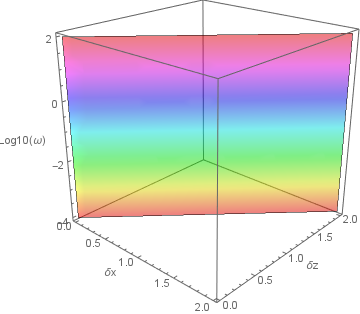
\includegraphics[width=1\linewidth]{FIGURES/Disp_Full_inner_00.png}
		\caption{}
	\end{subfigure}
	~
	\centering		
	\begin{subfigure}{0.36\linewidth}
		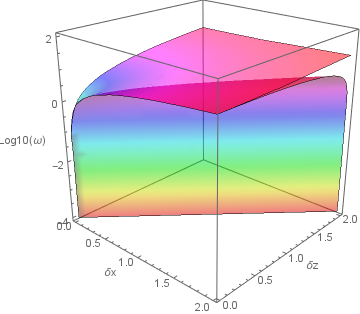
\includegraphics[width=1\linewidth]{FIGURES/Disp_Full_inner_10.png}
		\caption{}
	\end{subfigure}
	~
	\centering		
	\begin{subfigure}{0.36\linewidth}
		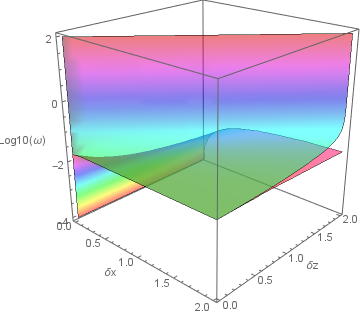
\includegraphics[width=1\linewidth]{FIGURES/Disp_Full_inner_01.png}
		\caption{}
	\end{subfigure}
	~
	\centering
	\begin{subfigure}{0.36\linewidth}
		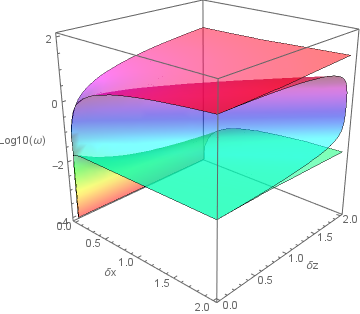
\includegraphics[width=1\linewidth]{FIGURES/Disp_Full_inner_11.png}
		\caption{}
	\end{subfigure}

	\caption{\textit{dispersion surfaces in $(\delta_x,\ \delta_z,\ Log_{10}(\omega))$ space and wave solutions for an homogeneous and incompressible ocean. Polychrome: inner dispersion surfaces:
	(a) $\epsilon_i=\epsilon_a=0$,
	(b) $\epsilon_i=0$,
	(c) $\epsilon_i=0$, 
	(d) $\epsilon_a=0$.}}
	\label{FigFullHomogeneous}
\end{figure}

%To identify regions of $(\delta_x,\ \delta_z,\ \omega)$ phase-space where the dispersion surfaces intersect and to further understand the physics of the waves corresponding to the intersections, wave solutions are successively studied in an homogeneous-incompressible, homogeneous-compressible and stratified-incompressible ocean before eventually focusing on a more realistic, stratified and compressible ocean.\\

%\subsubsection{Surface waves in an homogeneous, compressible ocean}
Figure \ref{FigFullHomogeneous} shows plots of the inner dispersion surface respectively for an homogeneous, incompressible ocean (figure \oldref{FigFullHomogeneous}.a), for an homogeneous, compressible ocean (figure \oldref{FigFullHomogeneous}.b), for a stratified, incompressible ocean (figure \oldref{FigFullHomogeneous}.c) and for a stratified, compressible ocean (figure \oldref{FigFullHomogeneous}.d). When not vanishing the acoustic and internal parameters $(\epsilon_a,\ \epsilon_i)$ are given in table \ref{TableParameters} for a reference ocean.

%%%%%%%%%%%%%%%%%%%%%%%%%%%
% Table  parameters
%%%%%%%%%%%%%%%%%%%%%%%%%%%
\begin{table}[h]
	%\centerline{
	\begin{tabular}{lll}
		Gravity&$g$&9.8 m.s$^{-2}$\\
		Sound speed&$c_s$&1500 m.s$^{-1}$\\
		Depth&$H$&4000 m\\
		Brunt-V\"ais\"al\"a frequency&$N$&10$^{-3}$ s$^{-1}$\\
		Compressible Brunt-V\"ais\"al\"a frequency & $N_c=\sqrt{N^2-g^2/c_s^2}$ & 9.6 10$^{-4}$ s$^{-1}$\\[4mm]
		Acoustic small parameter&$\displaystyle \epsilon_a=\frac{\sqrt{gH}}{c_s}$&$\approx 		0.132$\\[4mm]
		Internal small parameter&$\displaystyle \epsilon_i=\sqrt{\frac{N_c^2H}{g}}$&$\approx 				0.0193$\\[4mm]
		Scale depth&$D_0=1/\left(\frac{N^2}{g}+\frac{g}{c_s^2}\right)
		=\frac{H}						{\epsilon_a^2+\epsilon_i^2}$
		&$\approx 224$ km
	\end{tabular}
	%}
	\caption{Main parameters used to plot dispersion relations.}
	\label{TableParameters}
\end{table}
%%%%%%%%%%%%%%%%%%%%%%%%%%%
% Table 
%%%%%%%%%%%%%%%%%%%%%%%%%%%

%Figure (\oldref{FigFullHomogeneous}.a) shows the dispersion surface for large horizontal and vertical wave-numbers whereas (\oldref{FigFullHomogeneous}.b) corresponds to the same surfaces in the vicinity of the origin, i.e. for small horizontal and vertical wave-numbers.

Each dispersion relation induces a relation between the non-dimensional wave-numbers $(\delta_x,\ \delta_z)$ and the non-dimensional pulsation $\omega$. For vanishing $\epsilon_i$ and $\epsilon_a$ parameters, the inner dispersion surface is given by the inner dispersion relations \ref{EqFullDisperai} with pure imaginary vertical wave-numbers $\delta_z=i\delta_{z,i}$. The y-axis showing $\delta_{z,i}$. The inner dispersion surface for pure-imaginary wave-number is a vertical plane (figure \oldref{FigFullHomogeneous}.a). When $\delta_x$ and $\delta_{z,i}$ are both positive the equation of the inner dispersion surface is given by $\delta_x-\delta_{z,i} =0$ in agreement with the conclusions reached in Subsection \ref{subsubsectioniR}. For an homogeneous, incompressible ocean, no wave can propagate at the same time in the horizontal and vertical directions and the only waves which can propagate over the horizontal are vertically vanishing waves which only present an interest for a bounded ocean (see \ref{SectionGraphic}.
%These waves are surface waves propagating in an homogeneous, compressible, free-surface ocean, we shall see in Section \ref{SectionAnalyticalSol} that usual approximations of swell correspond to one point of this black-line intersection in phase-space.

%\subsubsection{Waves in a stratified or in a compressible ocean}
Figure (\oldref{FigFullHomogeneous}.b-d) further displays the inner dispersion surface for successively a homogeneous and compressible ocean. A comparison of figure (\oldref{FigFullHomogeneous}.a) with figures (\oldref{FigFullHomogeneous}.b-d) shows that when $\epsilon_a \neq 0$ the upper part of the inner dispersion surface folds. A new branch of the inner dispersion surface, this time for real $\delta_z$ appears in the upper region corresponding to large pulsations in such a way that waves can propagate for large pulsation $\omega$. In the same way, the lower part of this same figure folds when $\epsilon_i \neq 0$ and a new branch for real $\delta_z$ appears in the lower region, i.e. for small pulsations. None of the waves corresponding to the upper or lower surfaces satisfies the ocean surface and bottom boundaries. As a consequence they can only be solutions under an assumption of unbounded ocean, i.e. locally and far from these boundaries. The upper branch (for large pulsations) corresponds to acoustic waves whereas the lower branch (for small pulsations) describes internal wave rays. Both should be detailed in subsection \ref{SubSectionUsualDisp}.

This is consistent with the inner dispersion relation \ref{EqFullDisperai} which shows that the difference between $\delta_x$ and $\delta_{z,i}$ is proportional to both $\epsilon_i$ and $\epsilon_a$.

%One way to give a physical meaning to the various branches of the dispersion surfaces and to associate them to physical waves with real vertical wave-numbers is to compare these branches to the physically meaningful acoustic and stratification functions ($\omega_a$ and $\omega_i$) derived and discussed in previous section \ref{SectionDisp}. 

%The surfaces $\omega^2=\omega_a^2$ and $\omega^2=\omega_i^2$ can be drawn in \ref{FigFullHomogeneous} and appear to be visually indistinguishable from respectively the inner dispersion branch in the upper region of figure (\oldref{FigFullHomogeneous}.c) and in the lower region of figure (\oldref{FigFullHomogeneous}.e) (consequently not shown in \ref{FigFullHomogeneous}). This consequently confirms the results of Section \ref{SectionAnalyticalSol}:
%\begin{itemize}
%	\item \textit{if $\omega>>1$ and $\delta_z\in\mathbb{R}$}, $\omega_+^2\approx\omega_a^2$ and the upper branch of the inner dispersion surface is close to the surface $\omega^2=\omega_a^2$. Waves lying on this surface are \textit{acoustic waves}.
%	\item \textit{if $\omega<<1$ and $\delta_z\in\mathbb{R}$}, $\omega_-^2\approx\omega_i^2$ and the lower branch of the inner dispersion surface is close to the surface $\omega^2=\omega_i^2$. Waves lying in on this surface are \textit{gravity waves}.
%\end{itemize}
%In a bounded ocean, wave-solutions can be found at the intersection of the inner and boundary dispersion surfaces. Numerical approximations of these intersections are plotted with blue points for the acoustic waves and with red points for the internal waves in figures (\oldref{FigFullHomogeneous}.c and e). The resulting color lines show that both acoustic and internal waves additionally present a quantified vertical wave-number of the form $\delta_z=\pi/2+m\pi$ for acoustic waves and $\delta_z=n\pi$ for internal waves. The former are thus acoustic modes modified by stratification and shall now be called \textit{Modified Acoustic Modes (MAM)} whereas the latter are (well-known) internal modes modified by compressibility and shall now be called \textit{Modified Internal Modes (MIM)}.\\

%If now $\delta_z\in i\ \mathbb{R}$, Figures (\oldref{FigFullHomogeneous}.d) and (\oldref{FigFullHomogeneous}.f) show that for a compressible or a stratified ocean, the inner and boundary dispersion surfaces intersect and, even if the inner surfaces are not vertical planes any more, the form of the intersection black-lines only slightly differ from the black line on (\oldref{FigFullHomogeneous}.a). The ocean waves associated to this intersection are surface waves modified by ocean compressibility or stratification and shall now be called \textit{Modified Surface Waves (MSW)}.\\ 

\subsection{Approximation with factorizing functions $\omega_a$ \& $\omega_i$}
Figure \ref{FigOmega} shows the branches of the inner dispersion surface far from and close to the origin together with the surfaces $\omega^2=\omega_a^2$ and $\omega^2=\omega_i^2$ for a reference ocean (table \oldref{TableParameters}). For pure-imaginary vertical wave numbers, the inner dispersion surface is folded both for large and, for real vertical wave-numbers, small pulsations and the upper (acoustic) and lower (stratification) branches are present for large and small pulsations.\\
In the upper and lower regions, the acoustic and stratification branches cannot be distinguished from the (red and yellow) surfaces $\omega^2=\omega_a^2(\delta_z)$ and $\omega^2=\omega_i^2(\delta_z)$. The conclusions are however less straightforward for the middle-range branch of the inner dispersion surface for pure imaginary vertical wave-numbers. The upper and lower regions are still well-represented respectively by the acoustic and stratification factorizing functions $\omega^2=\omega_a^2(\delta_{z,i})$ (blue surface) and $\omega^2=\omega_i^2(\delta_{z,i})$ (green surface). In the middle-range regions (neighbourhood of the $\delta_x=\delta_{z,i}$ vertical plane) the approximation of the inner dispersion surface with the factorizing functions is much less accurate. Discrepancies are particularly large close to the origin in phase space, i.e. for long waves (figure \oldref{FigOmega}.b). In this middle-range  region, one could say that waves are both influence by compressibility and gravity. However a quick comparison with Figure \ref{FigFullHomogeneous} shows that the vertical part of the middle-range branch is rather similar to the inner dispersion plane $\delta_{z,i}=\delta_x$ obtained for an homogeneous, incompressible ocean. They are moreover badly described by either the acoustic or the stratification functions ($\omega_a$ or $\omega_i$). This would suggest that waves in this region are in fact only slightly influence by both stratification and compressibility as suggested in Subsection \ref{subsubsectioniR}.\\

In regions where they provide a good approximation, the acoustic and stratification factorizing functions can also help characterizing the geometry of the various branches of the dispersion surfaces. The form of the $(\omega^2=\omega_a^2)$ surface indicates indeed that the upper branch is an hyberboloid of two sheets but since $\omega^2=\omega_i^2$ is not a second-order polynomial due to the importance of the stratification-related $(\epsilon_i\ \delta_x^2 / \omega^2)$ term in \ref{EqFullDispera}, the lower cannot be a quadric. For $\delta_z\in i\mathbb{R}$, the middle-range branch is a more complex fourth-order surface, however, its upper part resembles locally to an hyperloid of one branch symmetric with respect to the $\delta_x = 0$ vertical plane as waves can propagate in both directions along the x-axis.\\


\begin{figure}[!h]
	\centering		
	\begin{subfigure}{0.45\linewidth}
		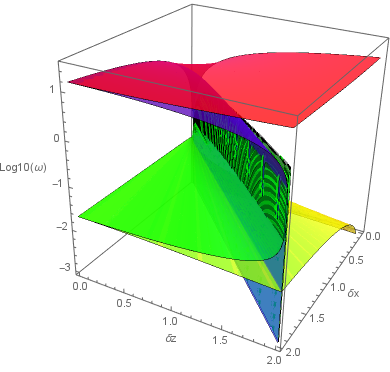
\includegraphics[width=1\linewidth]{FIGURES/Fig_omega.png}
		\caption{}
	\end{subfigure}
	~
	\centering		
	\begin{subfigure}{0.45\linewidth}
		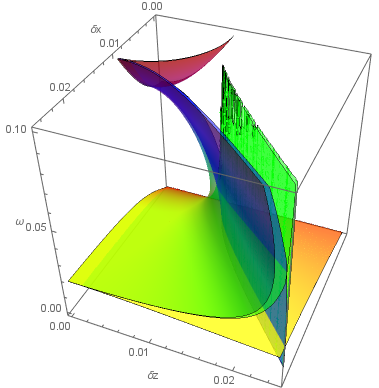
\includegraphics[width=1\linewidth]{FIGURES/Fig_omega_zoom.png}
		\caption{}
	\end{subfigure}
	~
	\caption{\textit{inner dispersion surface and factorizing functions $\omega_a$ and $\omega_i$. Polychrome: inner dispersion surface. Red: $\omega^2=\omega_a^2(\delta_x,\ \delta_z)$. Blue: : $\omega^2=\omega_a^2(\delta_x,\ i \delta_z)$. Green: $\omega^2=\omega_i^2(\delta_x,\ i \delta_z)$. Yellow: $\omega^2=\omega_i^2(\delta_x,\ \delta_z)$. (b) is a zoom of (a) in the vicinity of the origin.}}
	\label{FigOmega}
\end{figure}

\subsection{Wave solutions in an unbounded, incompressible ocean}
\label{SubSectionUsualDisp}

So far three types of solutions for the inner dispersion relation have been identified. Before investigating ocean waves interfering with the ocean upper and lower boundaries and satisfying the boundary dispersion relation \ref{EqFullDisperb}, we shall first show that traditional formulations of waves propagating in an "unbounded-ocean" can be recovered as Taylor approximations of previous wave solutions with $\delta_z\in\mathbb{R}$.\\
Indeed, in an "unbounded" ocean, waves only need to satisfy the "inner" dispersion relation \ref{EqFullDispera}. In a more realistic bounded ocean, such waves can exist if their vertical scales is (much) smaller than the ocean depth $(|\delta_z| << 1)$ and if they do not interfere with the bottom or the surface of the ocean. 
We shall additionally confirm in this simple configuration the physical meaning and the analytical importance of the factorization functions $\omega_a$ and $\omega_i$. 


\subsubsection{Modified internal waves (MIW)}

When $\delta_z\in \mathbb{R}$, a Taylor development of the gravity-wave root $\omega_{-}$ \ref{SolGrav} with respect to small parameters $\epsilon_a$ and $\epsilon_i$ leads to:
\begin{equation}
	\label{DispRaysDT}
		\frac{\omega_-^2}{\epsilon_i^2} =\underbrace{
		\frac{\delta_x^2}{\delta_x^2+\delta_z^2}
		\left(1-\frac{(\epsilon_i^2+\epsilon_a^2)^2}{4(\delta_x^2+\delta_z^2)}\right)}_{\approx\ \omega_i^2/\epsilon_i^2}
		+\frac{\epsilon_i^2\epsilon_a^2}{(\delta_x^2+\delta_z^2)^3}\delta_x^4
		+\mathrm{O}	(\epsilon_i^{6},\epsilon_a^{6})
\end{equation}
The traditional dispersion relation for dispersive internal gravity wave rays (\cite{gill_1982}, see also Table \oldref{TableWave solutions} above)
\begin{equation}
	\frac{\omega_{iwr}^2}{\epsilon_i^2}=\frac{ \delta_x^2}{\delta_x^2+\delta_z^2}
	\label{DispRays}
\end{equation}
is recovered at fourth order in $\epsilon_i$ and $\epsilon_a$. Relations \ref{DispRaysDT} and \ref{DispRays} further show that $\omega_{iwr}^2/\epsilon_i^2$ is a fourth-order approximation of $\omega_i^2/\epsilon_i^2$ and is itself an approximation of the general root $\omega_-^2/\epsilon_i^2$.
As a consequence, when parameters $\epsilon_i^2$ and $\epsilon_a^2$  are both small, the stratification function $\omega_i(\delta_x,\delta_z)$ is an internal gravity wave ray modified by compressibility and propagating in an unbounded ocean. Both corrective terms on the right-hand-side are proportional to $\epsilon_i^2+\epsilon_a^2=H/D_0$ and consequently depends on the relative strength of the stratification (with no compressibility correction). The first corrective term can only reduce the pulsation, the last term can only increase it. The ocean waves satisfying \ref{DispRaysDT} shall now be referred to as \textit{Modified Internal Waves (MIW)}.

\subsubsection{Modified acoustic waves (MAW)}

%If a real vertical wave-number is now associated to small-pulsation wave-solutions, we have shown in Subsection \ref{SubSectionDeltaz} that the pulsation was bounded by $\epsilon_i$. In dimensional form, this bound can be written $\Omega\leq N$ and can thus be related to well-known cut-off pulsation for internal gravity waves (Dukowicz, 2013).\\

If a real vertical wave-number is now associated to small-pulsation wave-solutions, a second-order Taylor development of the acoustic root $(\omega_+)$ with respect to $\epsilon_a$ and $\epsilon_i$ leads this time to:
\begin{equation}
		\epsilon_a^2\omega_+^2 =
		\underbrace{\delta_x^2+\delta_z^2
		+\frac{(\epsilon_i^2+\epsilon_a^2)^2}{4}}
		_{\approx\ \epsilon_a^2\omega_a^2}
		-\frac{\epsilon_i^2\epsilon_a^2\delta_x^2}{\delta_x^2+\delta_z^2}
		+\mathrm{O}(\epsilon_i^4,\epsilon_a^4)
		\label{DispAcousDT}
\end{equation}

The well-known dispersion relation for acoustic waves is thus recovered at order zero at the right-hand-side:
\begin{equation}
	\epsilon_a^2\omega_{aw}^2 =\delta_x^2+\delta_z^2
	\label{DispAcous}
\end{equation}

This expression is only modified at fourth order by small parameters $(\epsilon_i^2,\ \epsilon_a^2)$. Relations \ref{DispAcousDT} and \ref{DispAcous} show that $\epsilon_a^2 \omega_{aw}^2$ is a fourth-order approximation of $\epsilon^2 \omega_a^2$ which is itself a fourth-order approximation of the general root $\epsilon_a^2 \omega_+^2$.
For small parameters $(\epsilon_i^2,\ \epsilon_a^2)$, the acoustic function $\omega_a$ can thus be interpreted as an acoustic wave solution modified by the stratification of the ocean, through $\epsilon_i^2+\epsilon_a^2=H/D_0$. This modification is equal to $H/D_0$ and is a consequence of the linear advection term $-(c_s^2/D_0-g)\hat{\rho}_h w$ in Eq \ref{WM_d}. Ocean waves satisfying this time \ref{DispAcousDT} will be called \textit{Modified Acoustic Waves (MAW)} in the following.

%%%%%%%%%%%%%%%%%%%%%%%%%%%%%%%%%%%%%%%%%%%%%%%%%%%%%%%%%%%%%%%%%%%%%%%%%%%
\newpage
%%%%%%%%%%%%%%%%%%%%%%%%%%%%%%%%%%%%%%%%%%%%%%%%%%%%%%%%%%%%%%%%%%%%%%%%%%%
\section{Waves in a bounded ocean}
\label{SectionGraphic}
%%%%%%%%%%%%%%%%%%%%%%%%%%%%%%%%%%%%%%%%%%%%%%%%%%%%%%%%%%%%%%%%%%%%%%%%%%%

\subsection{Numerical investigation of MSW, MAM \& MIM}
\label{SubSectionPotBranches}

The compressible and stratified ocean is now supposed to be bounded. \\

\textit{Branches of the boundary dispersion surface:}\\
Figure \ref{FigDispSolutions} displays now simultaneously the inner and boundary dispersion surfaces for the same reference values of  $(\epsilon_i)$ and $(\epsilon_a)$ (table \oldref{TableParameters}). The branches of the boundary dispersion surface are first described before the intersections between the inner and boundary dispersion surface are computed numerically and plotted with color points. These intersections correspond to various wave solutions potentially propagating in a compressible, stratified, bounded ocean. Long waves (i.e. waves with small wave-numbers) are studied independently.

\begin{figure}[!h]
	\centering		
	\begin{subfigure}{0.45\linewidth}
		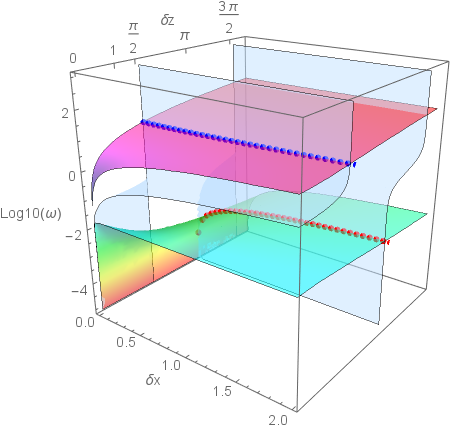
\includegraphics[width=1\linewidth]{FIGURES/Fig_Inter_Real.png}
		\caption{}
	\end{subfigure}
	~
	\centering
	\begin{subfigure}{0.45\linewidth}
		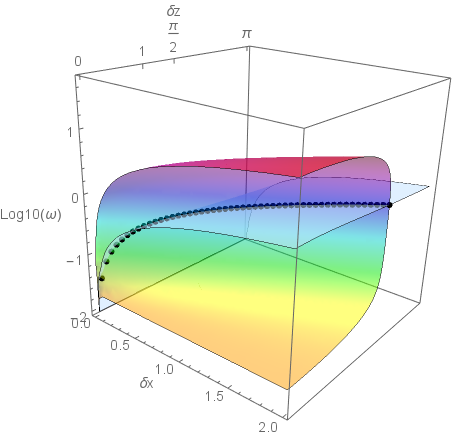
\includegraphics[width=1\linewidth]{FIGURES/Fig_Inter_Imag.png}
		\caption{}
	\end{subfigure}
	
	\begin{subfigure}{0.45\linewidth}
		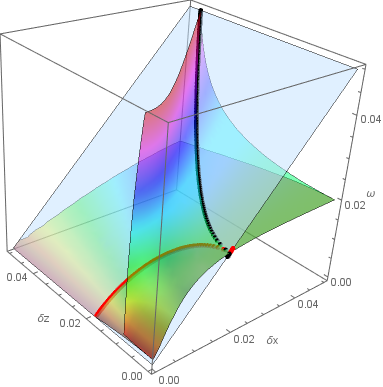
\includegraphics[width=1\linewidth]{FIGURES/Fig_Inter_All_zoom5.png}
		\caption{}
	\end{subfigure}
	~
	\begin{subfigure}{0.45\linewidth}
		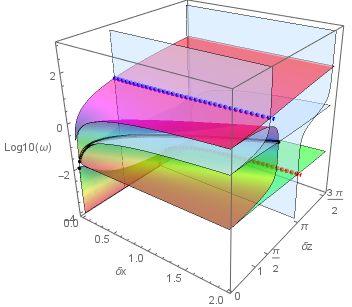
\includegraphics[width=1\linewidth]{FIGURES/Disp_Full_all.png}
		\caption{}
	\end{subfigure}

	\caption{\textit{dispersion surfaces in $(\delta_x,\ \delta_z,\ Log_{10}(\omega)$ or $\omega)$  space and wave solutions.\\
	 (a) Wave solutions with real $\delta_x$. Polychrome surfaces: Inner dispersion surface for real $\delta_z$ (acoustic and gravity branches). Blue: Boundary dispersion surface. Black points: acoustic wave (upper branch) and internal wave solutions (lower branch).\\
	 (b) Wave solutions with pure imaginary $\delta_x$. Polychrome surface: Inner dispersion surface for pure imaginary $\delta_z$ (surface gravity-wave branch). Blue: Boundary dispersion surface. Red points: surface wave solutions.\\ 
	 (c) Wave solutions in the vicinity of the origin. Polychrome surface: Lower (respectively upper) $\delta_x$: inner dispersion surface for real $\delta_z$ (pure imaginary $\delta_z$). Blue: Boundary dispersion surface. Black (red) points: surface wave solutions.\\
	 (d) Wave solutions with both real and pure-imaginary wave-numbers as given in (a) and (b). } }
	\label{FigDispSolutions}
\end{figure}
%For pure-imaginary vertical wave numbers, the inner dispersion surface is folded both for large and small pulsations. For real vertical wave-numbers branches are present in the upper and lower regions as could be expected by adding the transformations already observed in figure \ref{FigFullHomogeneous} when $\epsilon_i$ and $\epsilon_a$ were separately non zero. In the large-pulsation region, the upper branch of the inner dispersion surface is similar to figure (\oldref{FigFullHomogeneous}.c) and, once again, could not be distinguished from the $\omega^2=\omega_a^2$ surface. The same is true in the small-pulsation region where the lower branch of the inner dispersion surface could this time not be distinguished from the $\omega^2=\omega_i^2$ surface. This is a consequence of the separation of the roots of the inner dispersion relation \ref{solseq} or equivalently of the separation of the upper, acoustic and lower, acoustic branches already observed in figure \ref{FigFullHomogeneous}: when $\epsilon_i$ and $\epsilon_a$ are simultaneously non zero, MAW and MIW can simultaneously propagate. Nevertheless, relations \ref{DispAcousDT} and \ref{DispRaysDT} show that at higher order in this small parameters, their dispersion relations are modified by the stratification and/or the compressibility of the ocean. Figure \oldref{FigDispSolutions}.d additionally provides all dispersion surface branches on the same plot. It confirms inequality \ref{RelInequal}. The inner-dispersion surface for pure-imaginary wave-numbers is bounded by the same surfaces for real wave-numbers.\\
For real vertical wave-numbers firstly, the boundary dispersion-surface (light-blue surface) is a piece-wise vertical surface. It includes several branches: an asymptotic vertical branch which coincides with the trivial vertical plane $\delta_z=0$ (vanishing vertical wave-numbers, not shown for clarity) and piece-wise tangent-like vertical branches for $\delta_z \approx n\pi$ (small values of $\omega$) and for $\delta_z = \pi/2+m\pi$ (large values of $\omega$), with m and n two non-vanishing integer numbers. \\
For pure imaginary wave-numbers now, the light-blue surface looks like an horizontal hyperbolic-tangent-like surface. Figure \oldref{FigDispSolutions}.d shows that real and pure-imaginary boundary-dispersion surfaces are very close for small vertical wave-numbers and cannot be distinguished graphically. This is a consequence of the fact that the tangent and hyperbolic-tangent functions have similar first-order Taylor expansion (with respect to $\delta_z$ or $\delta_{z,i}$).\\

\textit{Numerical approximations of wave solutions in a bounded ocean:}\\
Figure \ref{FigDispSolutions} confirms in the general case the existing of three types of intersections between the inner and boundary dispersion surfaces and, as a consequence, three regions of phase-space where waves can propagate in a bounded ocean. These intersections are shown by three lines of color points. The black-point intersection corresponds to wave-solutions propagating with a pure imaginary vertical wave-number in the middle-range pulsation region (figures \oldref{FigDispSolutions}.b, c and d). These are surface (edge) waves propagating in a compressible, stratified ocean. Figure \oldref{FigDispSolutions}.d shows that they occupy a region of phase-space where the inner dispersion surface is approximately vertical and tangent to the $\delta_x\approx\delta_{z,i}$ plane meaning that the influence of compressibility and stratification (gravity) are both small. 

The red and blue lines of points indicates that two remaining wave-solutions are possible, this time with real vertical wave-numbers. One (blue points) is an intersection of the boundary dispersion surface with the upper acoustic branch of the inner dispersion surface (figures \oldref{FigDispSolutions}.a, c and d), the other (red points) is an intersection of the same boundary dispersion surface with the lower stratification branch of the inner dispersion surface (figures \oldref{FigDispSolutions}.a and d). Since in both cases, vertical wave-numbers are quantified ($\delta_z = \pi/2+m\pi$ and $\delta_z \approx n\pi$), the resulting wave solutions can be associated to respectively Modified Acoustic Modes (MAM) and Modified Internal Modes (MIM), these modes being modified by both compressibility and stratification (gravity).\\

\textit{Long-wave solutions:}\\
In the vicinity of the origin for  $(\mid\delta_x\mid <<1\  and\ \mid\delta_z\mid << 1)$ and for $(\mid\omega\mid <<1)$ (i.e. for large wave-lengths and large periods), the upper and lower branches of the inner boundary surface on one side and the boundary dispersion surfaces for $(\delta_z\in\mathbb{R})$ and $(\delta_z\in i\ \mathbb{R})$ on the other side intersect for $\delta_z=0$ in the small-pulsation region. The MAW and the MSW branches of the inner dispersion surface cannot be distinguished when $\delta_x$ and $\delta_z$ simultaneously tend toward 0 for larger pulsations (not shown in the phase-space region above figure (\oldref{FigDispSolutions}.c).\\
In this figure (\oldref{FigDispSolutions}.c), the black-point intersection is the continuation for small wave-numbers of the MSW intersection in figure (\oldref{FigDispSolutions}.b) whereas the red-point intersection is not connected to the MIM intersection shown in (\oldref{FigDispSolutions}.a). This continuous-by-part intersection leads to wave-solutions whatever $\delta_x$ in this region. For small values of $\delta_x$ the solution is given by the MIM branch (red points) whereas for larger values of $\delta_x$ it is given by the MSW branch (black points) and the vertical wave-number vanishes in between these solutions. Interestingly enough and contrary to the conclusions given by Dukowicz (2013), the barotropic mode pulsation cannot saturate at the buoyancy pulsation for increasing horizontal wave-number $(\delta_x)$ but transforms into a vertically evanescent surface-wave while its vertical number switches from real to pure imaginary. The resulting branch (in red) is an extension of the vertically evanescent wave solution presented in the previous section.\\
Figure (\oldref{FigDispSolutions}.a) also confirms that given $\delta_x$ and $\omega$ there exists a unique value of either $\delta_z$ or $\delta_{z,i}$ that satisfies the inner dispersion relation. The same is not true for $\delta_x$ or $\omega$ given this time $(\delta_z,\ \omega)$ or $(\delta_x,\ \delta_z)$. This confers a particular status to the vertical wave-number and confirms the choice made plotting Figure \ref{FigContourdz}. Duckowicz's figure 1 (Duckowicz, 2015) can be recovered by projecting dispersion surfaces on figure (\oldref{FigDispSolutions}.a) parallel to $\delta_z$ axis into the $\delta_z=0$ plane. Duckowicz's acoustic wave region (D), gravity wave region (A) and in between region (B, C, E and F) respectively correspond to MAM, MIM and MSW branches or surfaces. The present approach in 3D $(\delta_x,\ \delta_z,\ \omega)$ phase-space provides the possibilities to unfold the $\delta_z$ dependency. \\
%\section{Analytical approximation of surface, internal and acoustic wave-modes}
%\label{SectionAnalyticalSol}

\textit{Summary:}\\
Three types of wave solutions spreading on the three branches of the inner dispersion surface have thus been identified graphically: internal gravity (in a stratified ocean), acoustic (in a compressible ocean) and surface waves (in a free-surface ocean) are now successively investigated. Analytical expressions are systematically derived using Taylor developments of general roots $\omega_{\pm}$ with respect to small parameters $(\epsilon_i,\ \epsilon_a)$, simple approximations of wave dispersion relations. When necessary, asymptotic relations are derived with respect to $\delta_x$, $\delta_z$ or $\omega$. The Taylor developments additionally give indications on how usual wave solutions can be modified by gravity and the ocean stratification $(\epsilon_i)$ and/or by the ocean compressibility $(\epsilon_a)$. Table \ref{TableOrdersMag} additionally gives orders of magnitudes of the pulsation and length scales of the various wave solutions.

%\begin{figure}[!h]
%	\centering		
%	\begin{subfigure}{0.45\linewidth}
%		\includegraphics[width=1\linewidth]
%		{FIGURES/Fig_App3_Real_Acous.png}
%		\caption{}
%	\end{subfigure}
%	~
%	\centering
%	\begin{subfigure}{0.45\linewidth}
%		\includegraphics[width=1\linewidth]
%		{FIGURES/Fig_App3_Real_Grav_v2.png}
%		\caption{}
%	\end{subfigure}
%	
%	\begin{subfigure}{0.45\linewidth}
%		\includegraphics[width=1\linewidth]
%		{FIGURES/Fig_App4_Imag.png}
%		\caption{}
%	\end{subfigure}
%	~
%	\begin{subfigure}{0.45\linewidth}
%		\includegraphics[width=1\linewidth]
%		{FIGURES/Fig_App8_zoom.png}
%		\caption{}
%	\end{subfigure}
%	
%	\caption{\textit{approximations to MAW (a), MSW (b), MIW (c) and long modified waves (d). Polychrome: inner dispersion surfaces. Light-blue: boundary dispersion surfaces.\\
%MAM (blue lines): numerical approximation (solid), short waves $(\delta_{z,smam},\ \omega_{smam})$ (dash-dotted), long waves $(\delta_{z,lmam},\ \omega_{lmam})$ (dashed).\\
%MIM (red \& pink): numerical approximation (red, solid), MIM for $n=1$ $(\delta_{z,mim},\ \omega_{mim})$ (red,dashed), long MIM for  $n=1$ $(\delta_{z,lmim},\ \omega_{lmim})$ (red, dash-dotted), MIM for $n=0$ $(\delta_{z,mim},\ \omega_{mim})$ (pink, solid), long MIM for $n=0$ $(\delta_{z,lmimo},\ \omega_{lmimo})$ (pink, dotted).\\
%MSW (black): numerical approximation (solid), long waves $(\delta_{z,lmsw},\ \omega_{lmsw})$ (dashed), MSW-$\epsilon$ (dash-dotted). MSW (Grey): Swell $(\delta_{z,sw},\ \omega_{sw})$ (solid), long waves $(\delta_{z,lsw},\ \omega_{lsw})$ (dashed).} }
%	\label{Fig_Approx}
%\end{figure}

%%%%%%%%%%%%%%%%%%%%%%%%%%%
% Table order of magnitude
%%%%%%%%%%%%%%%%%%%%%%%%%%%
\begin{table}[h]
	%\centerline{
	\begin{tabular}{l|l|l|l|l}
		& \textit{Notation}   & \textit{Reference} & \textit{10-m-deep} & \textit{$N=10^{-2}\ s^{-1}$}\\\hline
		Parameters & $\epsilon_a$ &
		$1.3\  10^{-2}$ &
		$6.6\  10^{-3}$ & $0.13$\\
		& $\epsilon_i$ &
		$2.0\ 10^{-2}$ &
		$1.0\ 10^{-3}$ & $0.20$\\\hline
		Acoustic cut-off&$2\pi \sqrt{H/g} /\omega_{c,a}$ & $30\ mn$ & $30\ mn$ & $9.6\ mn$\\\hline
		Internal cut-off& $2\pi \sqrt{H/g} /\omega_{c,i}$& $1.7\ h$ & $1.7\ h$ & $10.5\ mn$\\\hline
		LMIM-LMSW cut-off & $2\pi H/\delta_{x,0}$& $1367\ km$ & $1000\ km$ & $123\ km$\\
		& $2\pi \sqrt{H/g} \omega_{x,0}$ & $1.9\ h$ & $1.7\ h$ & $10.5\ mn$\\\hline
		LMIM-$\delta_z(0)$ & $2\pi H/\delta_{z,0}$& $1379\ km$ & $62\ km$& $125\ km$\\
		& $2\pi \sqrt{H/g} \omega_{z,0}$ & $\infty$& $\infty$ & $\infty$\\ \hline
		MSW-neutral point & $2\pi H/\delta_{x,*}$& $161\ km$ & $407\ m$ & $123\ km$\\
		&$2\pi H/\delta_{z,*}$ & $164\ km$ & $407\ m$&$2148\ km$\\
		&$2\pi \sqrt{H/g} \omega_{*}$ &$12\ mn$&$41.3\ s$&$10.5\ mn$\\
	\end{tabular}
	%}
	\caption{orders of magnitude of various scales. Notations refer to non-dimensional variables whereas orders of magnitude are given for dimensional quantities. Parameters for the "\textit{Reference}" ocean are given in Table \ref{TableParameters}. "\textit{10-m-deep}" ocean is a  10-m-deep \textit{Reference} ocean and "$N=10^{-2}\ s^{-1}$" refers to a \textit{"Reference"} ocean with $N=10^{-2}\ s^{-1}$.} 
	\label{TableOrdersMag}
\end{table}
%%%%%%%%%%%%%%%%%%%%%%%%%%%
% Table +
%%%%%%%%%%%%%%%%%%%%%%%%%%%

%%%%%%%%%%%%%%%%%%%%%%%%%%%%%%%%%%%%%%%%%%%%%%%%%%%%%%%%%%%%%%%%%%%%%%%%%%%%%
\subsection{Surface-trapped acoustic-gravity waves}
\label{SubSectionGraphicMSW}
%%%%%%%%%%%%%%%%%%%%%%%%%%%%%%%%%%%%%%%%%%%%%%%%%%%%%%%%%%%%%%%%%%%%%%%%%%%%%
%In the present section, these approximations are plotted on figure \ref{Fig_Approx}to be compared with the correction numerical approximation obtained in Section \ref{SectionGraphic}.
"Surface waves" generally refer to wave propagating horizontally as anomalies of the ocean free-surface (\cite{gill_1982}). In the vertical direction, these surface wave anomalies are "evanescent" meaning that, with the notation chosen in the present study, the vertical wave-number $(\delta_z)$ is a purely imaginary complex number. An alternative way to introduce "surface waves" is to introduce them as a limiting case of internal gravity mode (Duckowicz, 2015): they are then referred to as a barotropic mode with mode-number "n = 0" (using the notations of Section \ref{SectionGraphic}). The numerical investigation of long MSW conducted in the previous subsection indicates that these two characterizations refer to two different wave solutions.\\
A MSW defined by its triplet $(\delta_x,\ \delta_z,\ \omega)$ must satisfy both the inner \ref{EqFullDispera} and boundary \ref{EqFullDisperb} dispersion relations for $\delta_z\ =\ i\ \delta_{z,i}$. A consequence is that the dispersion relations of these horizontally propagating waves, should, at least in theory, be advantageously parameterized in the form $(\ \delta_z(\delta_x),\ \omega(\delta_x)\ )$. As already stated before, such a parametrization is yet difficult to formulate since (i) the inner dispersion relation is fourth order in $\omega$ and (ii) the boundary dispersion relation is transcendental in $\delta_z$. A consequence is that analytically-simple, physically meaningful formulations can only be obtained under (very) restrictive assumptions.\\ 
%A way to circumvent these difficulties is to iteratively approximate and substitute $\delta_z(\delta_x)$ and $\omega(\delta_x)$ using both the inner and boundary dispersion relations.\\

\subsubsection{Swell-like approximation of MSW}

%In an homogeneous, incompressible ocean, both small parameters $\epsilon_i$ and $\epsilon_a$ vanish and we have shown in Section \ref{SectionGraphic} that the inner dispersion relations \ref{EqFullDispera} and \ref{EqFullDisperb} have a solution only for pure-imaginary vertical wave-numbers satisfying exactly $\delta_x=\delta_{z,i}$. In a stratified, compressible ocean, a MSW can propagate and the importance of stratification and/or compressibility can be evaluated by considering the difference $\delta_x-\delta_{z,i}$ (section \oldref{subsubsectioniR}).

For pure imaginary vertical wave-numbers, the inner dispersion-relation \ref{EqFullDisperai} shows that at zeroth order in small parameters $(\epsilon_a,\ \epsilon_i)$, the horizontal and vertical wave-numbers are approximately identical: $\delta_x^2=\delta_{z,i}^2+\mathrm{O}(\epsilon_i^2,\epsilon_a^2)$. This relation is often postulated in textbook to reduce the number of variables. Vertical polarization relations are then functions of $\delta_x$ only (\cite{gill_1982}) and, as a consequence, the deduced dispersion relation is the boundary dispersion relation \ref{EqFullDisperb} for pure imaginary $\delta_z$ or an approximation of this relation. In this case, $\delta_{z,i}$ is just the vertical length-scale for wave decrease downward from the surface and, for (very) long waves $\delta_x>>1$, the surface wave is thus approximately depth-independent and the vertical length-scale disappears.\\
We concluded in subsection \ref{subsubsectioniR} that Relation \ref{EqFullDisperai} gives the main corrective terms to this very crude first approximation: two terms  $\epsilon_i^2 \delta_x^2/\omega^2+(\epsilon_a^2+\epsilon_i^2)/4$ are associated to the stratification, one $\epsilon_a^2\omega^2$ is due to compressibility. The larger these terms, the larger the difference. In Subsection \ref{SubSectionPotBranches}, the corresponding intersection (black line) is located in the vertical region of the middle-range branch fig. \ref{Fig_Approx}. We shall now see that the crude $(\delta_x\approx\delta_z)$ assumption is sufficiently accurate to recover usual swell-like approximations (table \oldref{TableWave solutions}) but not the behaviour of long MSW observed in Section \ref{SectionGraphic}. An approximation of $\delta_x$ at second order in $\delta_z$ is thus derived and discussed. 

At second order in $(\epsilon_i,\ \epsilon_a)$, the inner dispersion relation \ref{EqFullDisperai} simplifies to:
\begin{equation}
	\label{Eqdzdx1}
	\displaystyle
	\delta_{z,i}(\delta_x) = \delta_{z,sw}(\delta_x)=\delta_x + O(\epsilon_i^2,\ \epsilon_a^2)
\end{equation}
where $\delta_{z,sw}$ is defined in non-dimensional form in Table \ref{TableWave solutions}. This crude (but usual) approximation can be substituted in the boundary dispersion relation \ref{EqFullDisperbi}, leading at lowest order in $(\epsilon_i,\epsilon_a)$ to:
\begin{equation}
	\label{EqDispLonga1}
	\displaystyle
	\omega^2=\omega_{sw2}^2(\delta_x) =\underbrace{\delta_x
	 tanh(\delta_{x})}_{\equiv\omega_{sw}^2}
	 \left(1-
	 \frac{\epsilon_i^2+\epsilon_a^2}{2}\frac{tanh(\delta_{x})}{\delta_x}
	 \right)
	 + \mathrm{O}(\epsilon_i^4,\epsilon_a^4)
\end{equation}
This relation can in turn be re-substituted in the inner dispersion relation \ref{EqFullDisperai} to obtain a more accurate approximation of the inner dispersion relation for $\delta_z$:
\begin{equation}
	\label{Eqdzdx2}
	\displaystyle
	\delta_{z,sw2}(\delta_x) = \delta_x\ 
	\left( 1-\frac{\epsilon_a^2-\epsilon_i^2}{2} \right)
	 + O(\epsilon_i^4,\ \epsilon_a^4)
\end{equation}

Note that no additional hypothesis on the triplet $(\delta_x,\ \delta_z,\ \omega)$ is required to derive this relation, meaning that it can be used to characterize surface gravity waves as long as $\epsilon_i$ and $\epsilon_a$ remains relatively small. In an homogeneous, compressible ocean (at zeroth order in $\epsilon_i$ and $\epsilon_a$), this relation simplifies in particular to the usual relation $\omega^2=\omega_{sw}^2 = \delta_x\ tanh(\delta_x)$.\\
%The swell-like relation $(\delta_{z,sw},\omega_{sw})$ and the higher-order approximation $(\delta_{z,sw2},\omega_{sw2})$ correspond to the dashed-grey and solid-grey curves in Figure \ref{Fig_Approx}. For large wave-numbers and pulsation, these two lines are indistinguishable from the numerical approximation of the MSW intersection (solid black line): swell-like approximations thus lead to a good approximation of short MSW. This is however not the case for long MSW as shown in Figure (\oldref{Fig_Approx}.d). 
For medium-range and large pulsations, the swell-like relation is a good approximation of the intersection of the inner and boundary dispersion surfaces: when plotted in phase-space, it is indeed indistinguishable from the numerical approximation found in section \ref{SectionInner} (not shown). For (very) small pulsations, the swell-like relation cannot however not be a good approximation since $\delta_{z,sw2}(0)=\omega_{sw2}(0)=0$ contradicting figure (\oldref{FigDispSolutions}.c): it is thus a poor approximation of the behaviour of very long waves.
%goes indeedthrough the origin contradicting the behaviour of long MSW in the region of phase-space. The higher-order approximation does not lead to an accurate approximation of the value of $\delta_x$ leading to a vanishing $\delta_z$: higher-order approximation is required.\\
The usual dispersion relation for (very) long surface waves with well-known $\sqrt{g H}$ phase-velocity (i.e. waves satisfying $\delta_z=\delta_{z_vlsw}=\delta_x$ and $\omega=\omega_{vlsw}=\delta_x$) can be recovered from the swell-like relation. \\
The dispersion relations (\oldref{EqDispLonga1} - \oldref{Eqdzdx2}) give a parameterization of the (square of the) pulsation and vertical wave-number as functions of the horizontal wave-number at high order in the small parameters $(\epsilon_a,\ \epsilon_i)$. Its main drawback is that it remains transcendental in the wave-number.\\

%If this Swell-like approximation of MSW is accurate for short wave, its main drawback is that it remains transcendental in the wave-number and, as a consequence, further developments remain complicated and require additional approximations. A first Taylor approximation of the dispersion relation \ref{EqDispLonga1} with respect of $\delta_x$ (i.e. for long-MSW or long-swell) can be carried out:
%\begin{equation}
%	\label{Eqwdx1}
%	\displaystyle
%	\omega(\delta_x) =  \underbrace{\delta_x}_{=\omega_{lsw}}\
% 	\left( 1-\frac{\epsilon_i^2+\epsilon_a^2}{4} \right) 
% 	+ O(\delta_x^3,\epsilon_i^2,\ \epsilon_a^2)
%\end{equation}
%This relation is to be taken with care and only its second order in $\epsilon_i$ and $\epsilon_a$ is accurate. The relation \ref{Eqwdx1} shows indeed that for non-vanishing $\epsilon_i$ and $\epsilon_a$,


%At lowest order in $\delta_x$ now, the usual dispersion relation for (very) long surface gravity waves (with $\sqrt{g H}$ phase-velocity) is recovered (see Table \oldref{TableWave solutions}). Th
%This sequence of approximations approaches the intersection computed numerically (black-point line in Fig. \oldref{FigDispSolutions}) for Taylor developments of higher order (Figure \oldref{Fig_Approx}) and for large wave-numbers and pulsations, however the region of small vertical (and thus small horizontal) wave-numbers remains badly resolved. The (very) long-wave approximation (grey-dashed line on Fig. \ref{Fig_Approx}.d) goes through the origin (the horizontal and vertical wave-numbers simultaneously vanish) contradicting Figure \oldref{FigDispSolutions}.c: no dependency in $(\epsilon_i,\ \epsilon_a)$ is indeed maintained in the relation $\omega=\omega_{lsw}$. As this very crude approximation is partly relaxed with the fourth-order dependency in $(\epsilon_i,\ \epsilon_a)$ (grey dashed-dotted line on Figure \oldref{Fig_Approx}.d), the vertical wave-number $(\delta_z)$ vanishes for a finite horizontal wave-number $(\delta_x)$ when $\epsilon_i$ is not zero but still doe not agree with the numerical approximation shown in Figure (\oldref{FigDispSolutions}.c).\\

\subsubsection{long surface waves ($\delta_{z,i}<<1$)}

\textit{Long Modified Surface Waves (LMSW):}\\
Swell-like relations do not provide an accurate modelling of the behaviour of long MSW. A more accurate description of this region of $(\delta_x,\ \delta_z,\ \omega)$ is required and figure (\oldref{FigDispSolutions}.d) suggests that a Taylor development with respect to $\delta_z$ should first be carried out. This means that the vertical attenuation scale of the wave remains large compared to the ocean depth. The Taylor approximation with respect to $\delta_z$ additionally annihilates the transcendental character of the dispersion relations and provides an analytical description of the behaviour of long surface waves:
\begin{equation}
	\label{Eqxxx}
     \omega(\delta_x,\ \delta_{z,i}) = 
     \omega_{lmsw}^2(\delta_x,\ \delta_{z,i}) = \frac{2}{3}\delta_x^2 
 		\frac{6-2\delta_{z,i}^2+3(\epsilon_i^2+\epsilon_a^2)}
 		{2+(\epsilon_i^2+\epsilon_a^2)^2}
 		+ \mathrm{O}(\delta_{z,i}^4)\\[3mm]
\end{equation}
This expression of $\omega^2$ can be substituted in the inner dispersion relation \ref{EqFullDisperai} without further approximation to obtain an analytical expression for $\delta_{z,i}$:
\begin{subequations}
	\begin{alignat}{2}
 		& \delta_{z,i}^2(\delta_x) &&=\delta_{z,lmsw}^2(\delta_x)\\[3mm]
		\label{EqDispDeltaz0}
 		& &&=\frac{3}{4}
 		\frac{
 		(2+\epsilon_a^2+\epsilon_i^2)
 		\left(
 		4\ \delta_x^2(2+\epsilon_i^2-\epsilon_a^2)
 		-8\epsilon_i^2-4\epsilon_a^2\epsilon_i^2
 		+2\epsilon_a^4-6\epsilon_i^4
 		+\epsilon_a^6-\epsilon_i^6
 		+\epsilon_a^4\epsilon_i^2
 		-\epsilon_a^2\epsilon_i^4
 		\right)
 		}
 		{-4\delta_x^2\epsilon_a^2
 		+\left(12(1+\epsilon_a^2+4\epsilon_i^2/3)
 		+2\epsilon_a^4+7\epsilon_i^4
 		+10\epsilon_a^2\epsilon_i^2
 		+\epsilon_a^4\epsilon_i^2
 		+2\epsilon_a^2\epsilon_i^4
 		+\epsilon_i^6 \right)
 		}
 	\end{alignat}
\end{subequations}
Note that 6th-order approximation is given to obtained an accurate-enough description of the transition region for small vertical wave-numbers. $\delta_{z,i}$ vanishes indeed for:
\begin{equation}
	\label{EqDispDeltazLim0}
	\delta_{x,lmsw}^2(\epsilon_i,\ \epsilon_a)=\frac{
	3(2+\epsilon_i^2+\epsilon_a^2)^2
	(4\epsilon_i^2+\epsilon_i^4-\epsilon_a^4)
	}
	{
	12(4-\epsilon_a^4+4\epsilon_i^2+\epsilon_i^4)
	}
\end{equation}
giving a lower bound for the surface wave solution. No Taylor development has been carried out with respect to $\epsilon_i$ and $\epsilon_a$ to provide an accurate description of the MSW. A parametric description for long MSW of the form $(\ \delta_z(\delta_x),\ \omega(\delta_x)\ )$ can be obtained by substituting \ref{EqDispDeltaz0} in \ref{Eqxxx}. A simpler parameterized relation $\omega^2(\delta_x)$ could additionally be obtained with a Taylor development with respect to $\epsilon_i$ and $\epsilon_a$.\\

\textit{Long Modified Internal Modes (LMIM0):}\\
For horizontal wave-number smaller than this lower bound, the graphical study carried out in section \ref{SectionGraphic} indicates that this MSW solution can be extended toward smaller horizontal wave-numbers by a gravity wave solution (MIM). The purely-imaginary vertical wave-number $\delta_z$ bifurcates in this case to a real value. Figure (\oldref{FigDispSolutions}.c) further indicates that for $\delta_x^2 \leq \delta_{x,lmsw}^2$, this solution is the intersection of the lower branch of the inner dispersion surface with the boundary dispersion surface providing an additional MIM solution for mode-number $n=0$. 
The inner and boundary dispersion relations \ref{EqFullDispera} and \ref{EqFullDisperb} for $\delta_z\in\mathbb{R}$ can be similarly expanded with respect to $\delta_z$ leading to:
\begin{subequations}
	\begin{alignat}{2}
	\label{MIMomega2}
     	& \omega_{lmim0}^2(\delta_x,\ \delta_z=i\delta_{z,i}) &&=
     	  \omega_{z,lmsw}^2(\delta_x,\ \delta_{z,i})\\[3mm]
	\label{MIMdz2}
 	 &\delta_{z,lmim0}^2(\delta_x) &&= -\ \delta_{z,lmsw}^2(\delta_x)
 	\end{alignat}
\end{subequations}
where $\delta_{z,lmsw}(\delta_x)$ is given by \ref{EqDispDeltaz0} and a parametric description of this MSW solution of the form $(\ \delta_z(\delta_x),\ \omega(\delta_x)\ )$ can similarly be obtained by substituting \ref{MIMomega2} into \ref{MIMdz2}. The resulting parametrization $(\delta_{z,mim}(\delta_x),\ \omega_{mim}(\delta_x))$ does not lead to a simple formulation of MIM for $\delta_z\approx0$ and it is consequently only plotted on Figure (\oldref{Fig_Approx}.d) with a pink-solid line. This line cannot be distinguished from the numerical solution (red-solid line). This approximation leads to an accurate representation of long MIM (for small $\delta_x$). The bifurcation point (where $\delta_z$ vanishes) is also well represented.\\
This long MIM branch intersects the $\delta_x=0$ plane for:
\begin{equation}
	\label{EqDispDeltaz0MIM}
 		\delta_{z,lmsw}^2(0)
 		=\frac{3}{4}
 		\frac{
 		(2+\epsilon_a^2+\epsilon_i^2)
 		\left(
 		8\epsilon_i^2+4\epsilon_a^2\epsilon_i^2
 		-2\epsilon_a^4+6\epsilon_i^4
 		-\epsilon_a^6+\epsilon_i^6
 		-\epsilon_a^4\epsilon_i^2
 		+\epsilon_a^2\epsilon_i^4
 		\right)
 		}
 		{
 		\left(12(1+\epsilon_a^2+4\epsilon_i^2/3)
 		+2\epsilon_a^4+7\epsilon_i^4
 		+10\epsilon_a^2\epsilon_i^2
 		+\epsilon_a^4\epsilon_i^2
 		+2\epsilon_a^2\epsilon_i^4
 		+\epsilon_i^6 \right)
 		}
\end{equation}

A simpler expression can be derived by expending the $(\ \delta_{z,lmim}(\delta_x),\ \omega_{lmim}(\delta_x)\ )$ parametrization with respect to $\delta_x$ and $\epsilon_i\ -\ \epsilon_a$. This leads to a long-wave approximation of LMIM of the form:
\begin{subequations}
	\begin{alignat}{2}
	\label{MIMomega}
	&\omega_{lmim00}(\delta_x) &&=\underbrace{\delta_x}_{\omega_{lsw}}\left(1-\frac{1}{4}\left(\frac{\epsilon_i^2}{3}+\epsilon_a^2\right)\right)
	 + \mathrm{O}(\delta_x^3,\epsilon_i^4,\epsilon_a^4)\\[3mm]
	\label{MIMdz}
	&\delta_{z,lmim00}(\delta_x) &&=\epsilon_i
	-\frac{1}{8}\left(\frac{\epsilon_a^4}{\epsilon_i}+\frac{\epsilon_i^3}{3}\right)
    +\delta_x^2\left(
    -\frac{1}{2\epsilon_i}+\frac{7\epsilon_i}{48}
    +\frac{\epsilon_a^2}{2\epsilon_i}-\frac{\epsilon_a^4}{16\epsilon_i^3}
    \right)
	 + \mathrm{O}(\delta_x^4,\epsilon_i^4,\epsilon_a^4)
   	\end{alignat}
\end{subequations}
%The resulting parameterizations $(\ \delta_{z,lmim}(\delta_x),\ \omega_{lmim}(\delta_x)\ )$ and $(\ \delta_{z,lmim0}(\delta_x),\ \omega_{lmim0}(\delta_x)\ )$ are plotted in (\oldref{Fig_Approx}.c) with respectively a pink-solid line and a pink-dashed line. None of lines can be distinguished from the numerical approximation of MIM (red-solid line) in the vicinity of $\delta_x=0$. However, not surprisingly, only the first parameterization (LMIM) gives an accurate description of the bifurcation point $(\delta_z=0)$.\\
The expressions for (very) long surface wave with $\sqrt{gH}$ phase-velocity can only partly be recovered for small $\epsilon_i$ and $\epsilon_a$. Indeed, at lower order $\omega^2\approx\delta_x^2$ but Relation \ref{MIMdz2} implies that $\delta_z\neq\delta_x$.\\

\textit{Physical interpretation:}\\
%For small horizontal wave-number, the wave solution can be viewed as a (long) \textit{barotropic mode} $(n=0)$ since it is on the same inner dispersion branch as MIM which are solutions for $n>0$. 
In an homogeneous ocean (whether compressible or not), the lower branch of the inner dispersion surface disappears (figure \oldref{FigFullHomogeneous}.d): the existence of the long (mode-0) MIM solution in the vicinity of the origin is thus a consequence of the stratification of the ocean. Note that an homogeneous ocean is obtained by setting to zero the stratification parameter $\epsilon_i$ together with the last (advective) term on the right-hand-side of the inner dispersion relation \ref{EqFullDispera}: $-(\epsilon_i^2+\epsilon_a^2)^2/4$. When the horizontal wave-number of a (short) MSW is reduced (i.e. its wave-length is increased) in a stratified, compressible ocean, the influence of the stratification increase due to the presence of this lower branch of the inner dispersion surface.  
MSW are yet primarily edge wave: the free-surface anomaly is one way or the other translated into a pressure anomaly by gravity, wave propagation is then achieved by a simple compensation mechanism based on the conservation of mass and momentum. If the ocean is homogeneous and incompressible, the pressure is an harmonic function and the horizontal and vertical length-scales have no reason to differ $(\delta_x=\delta_z)$. Compressibility and stratification modifies this and we already discussed in Section \ref{subsubsectioniR} that, in this case, the difference between the horizontal and vertical wave-number increases. The vertical wave-number decreases consequently faster and the MSW variations become very small over the vertical. If $\delta_x$ is further decreased, $\delta_z$ finally vanishes for small but finite $\delta_x$.\\
If the horizontal wave-number keeps on decreasing, a surface wave can only propagate as a mode-0 (barotropic) MIM. In this case, the vertical wave-number must increase for a decreasing horizontal wave-number due to the stratification barrier: the stronger the stratification, the shallower the in-depth penetration of the surface wave.\\
We can finally note for an homogeneous ocean, the evanescent surface wave solution is valid till the origin where $\delta_z$, $\delta_x$ and $\omega$ all vanish. In an homogeneous ocean, the \textit{barotropic mode} $(n=0)$ does not exist and the inner dispersion surface does not intersect the boundary dispersion surface in the vicinity of the origin: the horizontal and vertical wave-numbers of the barotropic MSM simultaneously vanish. \\

\textit{Orders of magnitudes:}\\
For the 4000-m-deep reference ocean (Table \oldref{TableParameters}), the horizontal length scale associated to the transformation of the MSW into the long MIM $(\lambda_{x,lmsw}=2\pi/(\delta_{x,lmsw}/4000))$ reaches $1367\ km$ against $62\ km$ for the same 10-m-deep ocean. When $\delta_x$ keeps on decreasing below $\delta_{x,lmsw}$, $\delta_z$ increases monotically to a maximum value $\delta_{z,lmsw}(\delta_x=0)$. This vertical length scale reaches $1379\ km$ for the 4000-m-deep reference ocean and $62\ km$ for the same 10-m-deep ocean. The longer the horizontal length scale of the oscillation, the shorter the vertical length scale and the weaker the stratification (vanishing $\epsilon_i$) the longer the horizontal length-scale $\lambda_{x,lmsw}$. This long MIM solution is a low-frequency oscillation of the ocean due gravity and associated to the stratification of the ocean. It disappears when the stratification vanishes and the ocean can be assimilated to an homogeneous layer of water. It does persist in an incompressible ocean but is slightly modified by compressibility.


%
%%%%%%%%%%%%%%%%%%%%%%%%%%%%%%%%%%%%%%%%%%%%%%%%%%%%%%%%%%%%%%%%%%%%%%%%%%%%%
\subsection{Internal-gravity modes modified by compressibility (MIM)}
\label{SubSectionGraphicMIW}
%%%%%%%%%%%%%%%%%%%%%%%%%%%%%%%%%%%%%%%%%%%%%%%%%%%%%%%%%%%%%%%%%%%%%%%%%%%%%

%\subsection{Solutions refinement}
The upper (acoustic) and lower (gravity) branches of the inner dispersion surface for real $\delta_z$ are well-separated and the MAM and MIM solutions can thus be studied independently. The mode-0 (barotropic) MIM solution has already been studied in the previous section and, as a consequence, only solutions for large vertical wave-numbers needs to be investigated.\\
Waves can propagate horizontally between the bottom and surface of the ocean as in a wave guide. Internal gravity modes are well-known examples (\cite{gill_1982}). They must satisfy both the boundary dispersion-relation \ref{EqFullDisperb} and the inner dispersion relation \ref{EqFullDispera}. In the previous section, graphical inspections of wave solutions confirmed that gravity waves with quantified vertical wave-numbers could be found at the intersection of the inner and boundary dispersion surfaces (numerical solution shown with a red line on figure (\oldref{FigDispSolutions}.a).
We have also shown in Section \ref{SectionInner} that the root of the inner dispersion relation corresponding to internal gravity waves is well-approximated by $\omega_i^2$. This root can be substituted in the boundary dispersion relation \ref{EqFullDisperb} to obtain
\begin{equation}
	   \label{DispSysIntModesab}
		\omega^2(\delta_x) \approx\omega_i^2\implies
		\frac{\delta_x^2}
		{\delta_z/\tan(\delta_z)+\frac{\epsilon_i^2+\epsilon_a^2}{2}}
		\approx
		\frac{\epsilon_i^2 \delta_x^2}{\delta_x^2
		+\delta_z^2+\frac{1}{4}\left(
		\epsilon_i^2+\epsilon_a^2\right)^2}
		%=\frac{\delta_x^2\tan(\delta_z)}
		%{\delta_z+\frac{\epsilon_i^2+\epsilon_a^2}{2}\tan(\delta_z)}
\end{equation}
Since the right-hand-side decreases fast with $\delta_x$ and $\delta_z$, the vertical wave-number $\delta_z$ has to be close to $n\pi$ with $n$ a non-zero integer. This agrees with the internal gravity wave solution found graphically in Section \ref{SectionGraphic}.\\
A Taylor development of relation \ref{DispSysIntModesab} with respect to $\delta_z$ is required in the vicinity of $\delta_{z,n}^0=n\pi$ to obtain an analytical relation of the form $\delta_z(\delta_x)$ and the pulsation can finally be expressed as a function of $\delta_x$ using the expression of the stratification function $\omega_i$:
\begin{subequations}
	\begin{alignat}{2}	
	\label{ParamallMIM1}
	&\delta_{z}(\delta_x) &&=\delta_{z,mim}(\delta_x)=
	\underbrace{\delta_{z,n}^0}_{\delta_{z,im}}
	\left(
	1+\frac{\epsilon_i^2}{\delta_x^2+\delta_{z,n}^2}
	%+\frac{(\delta_x^2-\delta_{z,n}^2)}{(\delta_x^2+\delta_{z,n}^2)^3}\epsilon_i^4
	\right)
	+\mathrm{O}	(\epsilon_i^4,\epsilon_a^4)\\[3mm]
	\label{ParamallMIM2}
	&\omega^2(\delta_x) &&=\omega_{mim}^2(\delta_x)=
	\underbrace{\epsilon_i^2}
	_{\omega^2_{im}}
	\frac{\delta_x^2}{\delta_x^2+\delta_{z,n}^2}
	\left(1-\frac{2\epsilon_i^2\delta_{z,n}^2}{(\delta_x^2+\delta_{z,n}^2)^2}\right)
	+\mathrm{O}	(\epsilon_i^6,\epsilon_a^4)
	\end{alignat}
\end{subequations}
where $\delta_{z,im}$ and $\omega_{im}$ are defined in dimensional form in Table \ref{TableWave solutions}. This shows that the internal gravity modes are robust to compressibility since there is no dependency to $\epsilon_a$ at orders lower than 4 vanishes. This agrees with the separation of the roots $\omega_\pm$ of the inner dispersion relation for real vertical wave-numbers.\\
A simpler parametric relation can further be found in the vicinity of $\delta_z=\pi\ (n=1)$ in the long-wave limit using a Taylor development for vanishing $\delta_x$, $\epsilon_i$ and $\epsilon_a$:
\begin{subequations}
	   \label{EqParamInt}
	\begin{alignat}{2}	
	   \label{ParamMIM1}
	   %
		& \delta_z(\delta_x)=\delta_{z,lmim\pi}(\delta_x) &&= 
		\pi+\frac{\epsilon_i^2}{\pi} \left(
		1-\frac{\delta_x^2}{\pi^2} \right)
		+\mathrm{O}	(\delta_x^4,\epsilon_i^4,\epsilon_a^4)\\[3mm]
		%
	   \label{ParamMIM2}
		& \omega(\delta_x)=\omega_{lmim\pi}(\delta_x) &&=\frac{\epsilon_i}{\pi} \delta_x
		\left( 1
		-\frac{\delta_x^2}{2\pi^2} \right)
		+\mathrm{O}	(\delta_x^5,\epsilon_i^3,\epsilon_a^3)
	\end{alignat}
\end{subequations}
For a vanishing horizontal wave-number, these parametric relations show that the pulsation vanishes too but the vertical wave-number is not exactly equal to $\pi$ but to $\pi+\epsilon_i^2/\pi$. As a consequence, $\delta_z$ varies with the square of the stratification parameter $(\epsilon_i)$.\\
%This approximate solution is plotted in figure (\oldref{Fig_Approx}.b) (red dash-dotted line) together with the MIM approximation $(\ \delta_{z,mim}(\delta_x),\ \omega_{mim}(\delta_x)\ )$ (red dashed line). The latter MIM approximation cannot be distinguished from the numerical solution.

%
%%%%%%%%%%%%%%%%%%%%%%%%%%%%%%%%%%%%%%%%%%%%%%%%%%%%%%%%%%%%%%%%%%%%%%%%%%%%%
\subsection{Acoustic Modes modified by gravity (MAM)}
\label{SubSectionGraphicMAW}
%%%%%%%%%%%%%%%%%%%%%%%%%%%%%%%%%%%%%%%%%%%%%%%%%%%%%%%%%%%%%%%%%%%%%%%%%%%%%
%\subsection{Compressible zero-gravity ocean}
%In the particular case of zero-gravity ocean ($\epsilon_i = 0$), the dispersion relations %(\ref{EqFullDisper}) simplify to:

%\begin{subequations}
%	\begin{alignat}{2}	
 %		& \delta_x^2+\delta_z^2 &&=\epsilon_a^2 (\omega^2-\frac{1}{4})\\
%		& \omega^2 &&=\frac{\delta_x^2\ tan(\delta_z)}
%		{\delta_z+\frac{\epsilon_a^2}			{2}tan(\delta_z)}
%		=\frac{\delta_x^2}{\frac{\epsilon_a^2}{2}+\delta_z cotan(\delta_z)}
%	\end{alignat}
%\end{subequations}

\textit{Smith-like MAM (large pulsations)}\\
In Section \ref{SectionGraphic}, a numerical approximation of the intersection of the inner and boundary dispersion surfaces has been computed and plotted (blue line in figure \oldref{FigDispSolutions}). This intersection has been associated to Modified Acoustic Mode (MAM). An analytical parametrization is now derived for MAM with an iterative method and its characteristics are further investigated. Assuming that $\delta_z(\omega)\approx\delta_{z,m} \equiv \pi/2+m\pi$, a first approximation of $\delta_x^2(\omega)$ can be found based on a Taylor expansion with respect to $\epsilon_i$ and $\epsilon_a$:
\begin{equation}
    \delta_{x}^2(\omega) = \underbrace{\epsilon_a^2\omega^2
    -\delta_{z,m}^2\left(1+\frac{1}{\omega^2}\right)}_{\equiv\delta_{x,smith}^2(\omega)}
    	+\mathrm{O}	(\epsilon_i^4,\epsilon_a^4)
\end{equation}
Smith's expression (2.10) (\cite{smith_2015}) for the horizontal wave-number of such a mode is recovered. This first approximation can be substituted in a second-order Taylor expansion of the boundary dispersion relation \ref{EqFullDisperb} to obtain a more accurate approximation of $\delta_z(\omega)$. Its Taylor expansion (i) for large $\omega$ and (ii) for small parameters $(\epsilon_i^2,\ \epsilon_a^2)$ leads to:
\begin{equation}
	\label{paramMAM1}
	\delta_{z}(\omega)=\delta_{z,mam}(\omega) = 
	\underbrace{\delta_{z,m}\left(1+\frac{1}{\omega^2}\right)}_{\equiv\delta_{z,smith}}
	+\frac{\epsilon_i^2-\epsilon_a^2}{2\delta_{z,m}}\left(1-\frac{1}{\omega^2} \right)
	+\mathrm{O}	(\epsilon_i^4,\epsilon_a^4)
\end{equation}
where $\delta_{z,smith}$ is also defined in dimensional form in Table \ref{TableWave solutions}. This relation agrees with the acoustic-gravity modes derived by \cite{smith_2015} (first two terms of the above relation correspond to Smith's relation (2.9)). It additionally shows that these modes are not modified bellow order 4 in $\epsilon_i$ by the stratification and gives the second order dependency in $\epsilon_a$.\\
A more accurate approximation of $\delta_x^2(\omega)$ can further be calculated by once again substituting $\delta_z(\omega)$ in the inner dispersion \ref{EqFullDispera} leading to:
\begin{equation}
	\label{paramMAM2}
	\delta_x^2(\omega)=\delta_{x,mam}^2(\omega) = \epsilon_a^2\omega^2
	-\delta_{z,m}^2\left(1+\frac{2}{\omega^2}\right)
	+\epsilon_a^2\left(1-\frac{1}{\omega^2}\right)
	-\epsilon_i^2\left(1+\frac{\delta_{z,m}^2-1}{\omega^2}\right)
	+\mathrm{O}	(\epsilon_i^4,\epsilon_a^4)
\end{equation}
This latter expression shows a second-order dependency of the squared pulsation in the stratification parameter $\epsilon_i$. Following \cite{smith_2015}, it has been derived using a Taylor expansion for large $\omega$ meaning that it is relevant only to short acoustic modes.\\

\textit{Short and long wave approximations of MAM (parametrization)}\\

Approximated parametrizations can be found directly for MAM with large pulsation (LMAM) or small horizontal wave-number (SMAM). Two regions of phase space, and thus two physical behaviours, can indeed be distinguished. In the vicinity of the origin first $\delta_z$ and $\omega$ can be expressed as functions of $\delta_x$ and of the parameters $(\epsilon_i,\ \epsilon_a)$:
\begin{subequations}
	\label{ParamAcousModes1}
	\begin{alignat}{2}	
	   %
		\label{ParamLMAM1}
		&\delta_{z}(\delta_x)=\delta_{z,lmam}(\delta_x) &&= \delta_{z,m} 
		-\frac{\epsilon_a^2}{\delta_{z,m}^3}\delta_x^2
	+\mathrm{O}	(\delta_x^4,\epsilon_i^4,\epsilon_a^4)\\[3mm]
	%
		\label{ParamLMAM2}
	    &\omega(\delta_x)=\omega_{lmam}(\delta_x) &&= \frac{\delta_{z,m}}{\epsilon_a}
	    +\frac{\delta_x^2}{\delta_{z,m}\epsilon_a} 
	    \left(2
	    -\frac{\epsilon_a^2}{\delta_{z,m}^2} \right)
	    %+\delta_x^4 \left(\frac{16\epsilon_a}{\pi^5}
	    %-\frac{1}{\pi^3\epsilon_a} \right)
	    +\mathrm{O}	(\delta_x^4,\epsilon_i^3,\epsilon_a^3)
	\end{alignat}
\end{subequations}

%Far from the origin and for large pulsations, another parametric expression can be obtained for modified acoustic waves. Expressions are this time parametrized by the pulsation $(\omega)$:
%\begin{subequations}
%	   \label{ParamAcousModes2}
%	\begin{alignat}{2}	
%		\label{ParamSMAM1}
%		&\delta_{x}(\omega)=\delta_{x,smam}(\omega) &&= \epsilon_a \omega
%		+\frac{1}{2\omega\epsilon_a}\left( 
%		\epsilon_a^2-\epsilon_i^2-\frac{\pi^2}{4}
%		\right)
%		+\mathrm{O}	(\omega^{-3},\epsilon_i^4,\epsilon_a^4)
%		\\[3mm]
%		\label{ParamSMAM2}
%		&\delta_{z}(\omega)=\delta_{z,smam}(\omega) &&= \frac{\pi}{2}
%		+(\epsilon_a^2-\epsilon_i^2)
%		\left(-\frac{1}{\pi}
%		+\frac{1}{\omega^2}\left(
%		\frac{\pi}{2}-\frac{2}{\pi}\right)
%		\right)
%		+\mathrm{O}	(\omega^{-3},\epsilon_i^4,\epsilon_a^4)
%	\end{alignat}
%\end{subequations}

%Both parameterizations are shown on figure (\oldref{Fig_Approx}.a): the Taylor approximation for small $\delta_x$ is plotted with a blue, dash-dotted line whereas the Taylor approximation for large $\omega$ is plotted with a blue, dotted line. Figure (\oldref{Fig_Approx}.a) gives an idea of the domain of validity of each approximations. Smith's relation (\cite{smith_2015}) for such waves is an approximation of the second type i.e. for large $\omega$. We have additionally shown that MAM can also propagate as long waves. Both approximations have approximately the same vertical wave-number $(\delta_z \approx \pi/2)$ but a different horizontal wave-number $(\delta_x)$ and a different pulsation $(\omega)$.
MAM cannot propagate for (very) low frequency due to the acoustic cutt-off pulsation $\omega_{c,a}$ (subsection \oldref{SubSectionDeltaz}). Bellow this pulsation, MSW and MIM can still propagate in a bounded ocean.

%The cut-off pulsation can be obtained from the inner dispersion relation \ref{EqFullDispera} for $\delta_x=\delta_z=0$:

%\begin{equation}
% 	\displaystyle
% 	\label{MAM_cutoff}
%	\omega_{mam,0}=\frac{(\epsilon_i^2+\epsilon_a^2)^2}{4\epsilon_a^2}
%\end{equation}


\subsection{Close-to-singular MSW}

The condition for propagation $(\displaystyle R^2(\delta_x,\delta_z)\le \frac{1}{4})$ derived in Section \ref{SubSectionFactoDisp} has so far been left out. For pulsation $\omega$ to remain real in the inner dispersion relation \ref{EqFullDispera}, it must yet be satisfied.  This condition is automatically satisfied for real horizontal and vertical wave-numbers but not necessarily for pure-imaginary vertical wave-numbers.\\
A further question is to figure out if the resulting MSW wave solution can or cannot approach a region of the $(\delta_x,\ \delta_z,\ \omega)$ space where this condition is not satisfied. This would indeed lead to a pair of complex roots to \ref{solseq} and as a consequence to a wave solution diverging in time. Figure \ref{FigDelta} partially answers the question since it shows that the inner dispersion surface for pure-imaginary $\delta_z$ does not intersect the vertical (green) plane but it remains tangent to it. We can show that the vertical component of the normal to the inner dispersion surface (i.e. $\partial$\ref{EqFullDisperai} $/\partial \omega$ ) vanishes for:
\begin{subequations}
	\begin{alignat}{2}	
	   %\label{ParamAcousModes2}
		 \delta_x^2 - \delta_{z,i} ^2 
		+\frac{(\epsilon_i^2+\epsilon_a^2)^2}{4}
		-2 \epsilon_a^2 \omega^2 = 0
		\label{EqTurnPoints}
	\end{alignat}
\end{subequations}
	
\begin{figure}[!h]
	\centering		
	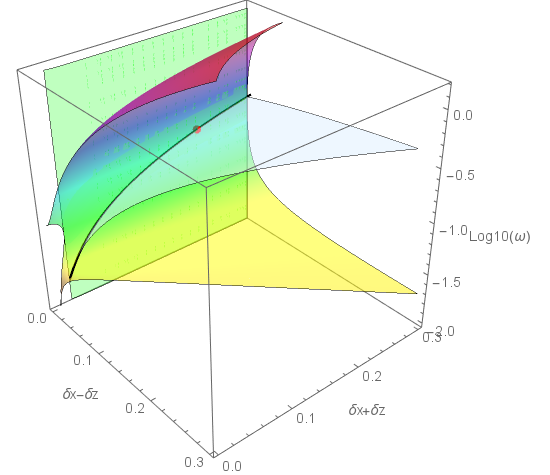
\includegraphics[width=0.5\linewidth]{FIGURES/Fig_Delta.png}
	\caption{\textit{region of SMW close to instability (pure-imaginary vertical wave-number). Polychrome: inner dispersion surface. Light-blue: boundary dispersion surface. Light-green: vertical surface tangent to the inner dispersion surface. Red point: SMW solution close to instability. }}
	\label{FigDelta}
\end{figure}


This set of points of the inner dispersion surface satisfies $\displaystyle R^2(\delta_x,i \delta_{z,i})= \frac{1}{4}$ and, as a consequence,
$\omega^2=\omega_a^2/2$. They correspond to the black line on Figure \ref{FigDelta}. This line separates the inner dispersion surface in two parts: the upper acoustic region $(\omega^2\approx\omega_a^2)$ closer to the MAM branch and the lower region $(\omega^2\approx\omega_i^2)$ closer to the MIM region.\\
We can then wonder if the MSW wave solution intersect this line of points, i.e. if wave solutions satisfying \ref{EqTurnPoints} and \ref{EqFullDisperai} can be found or not. Such an intersection exists if at least one point belongs to the boundary dispersion surface given by \ref{EqFullDisperb} or equivalently if the system of equations \ref{EqTurnPoints}, \ref{EqFullDisperai} and \ref{EqFullDisperb} has a solution. Only one point satisfies this system and is indicated by a large red dot on \ref{FigDelta}. Its horizontal and vertical wave-numbers can be expressed as functions of its pulsation:
\begin{subequations}
	\begin{alignat}{2}	
	   \label{ParamSolDelta}
	   &\delta_{z,i}(\omega) && =\frac{1}{2} 
	   \sqrt{(\epsilon_i^2+\epsilon_a^2)^2 
	   - 8 \epsilon_a^2 \omega^2
	   + 4 \frac{\epsilon_a^2}{\epsilon_i^2} \omega^4}\\[3mm]
	   &\delta_x(\omega) &&=\omega
	   \sqrt{\frac{\epsilon_a^2+\epsilon_i^2}{2}
	   +\delta_{z,i}(\omega)\ coth(\delta_{z,i}(\omega))}
	\end{alignat}
\end{subequations}
The pulsation $\omega$ must then be a solution of the (transdental) equation inherited from the inner dispersion relation \ref{EqFullDisperai}:
\begin{subequations}
	\begin{alignat}{2}	
	   \label{ParamSolDelta2}
 		\delta_x^2(\omega)-\delta_{z,i}^2(\omega) 
 		-\epsilon_i^2\ \frac{\delta_x^2(\omega)}
 			{\omega^2}-\epsilon_a^2\omega^2
 		+\frac{\epsilon_a^2+\epsilon_i^2}{4} = 0
	\end{alignat}
\end{subequations}
For the parameters $\epsilon_i$ and $\epsilon_a$ given in Table \ref{TableParameters}, this latter equation has only one solution for $\omega^*$ satisfying the system of equations \ref{EqTurnPoints}, \ref{EqFullDisperai} and \ref{EqFullDisperbi}. It can be evaluated numerically:
\begin{equation}
	\omega_* \approx 0.154
\end{equation}
Orders of magnitude of the wave-numbers $(\delta_{x,*},\ \delta_{z,*})$ and pulsations $(\omega_*)$ are given in Table \ref{TableOrdersMag}. The resulting wave solution is a MSW wave that satisfies $R^2(\delta_{x,*},\ \delta_{z,*})=1/4$. Graphically this means that the solution point (in red) belongs to the line of points with horizontal normal vector or vanishing vertical gradient with respect to $\omega$. Dynamically, this means that the corresponding wave solution is "on the edge" and that for a small variation of the wave-number, of the pulsation or one the parameters it may enters in the region of unstable waves satisfying $R^2>1/4$. \\
Other reference parameters given in Table \ref{TableParameters} remaining constant, Table \ref{TableOrdersMag} shows that when changing the depth of the reference ocean (4000 m) to only 10 m, the (normalized) pulsation $\omega_*$ remains quasi-constant and, as a consequence, the pulsation $\Omega_*$ varies approximately with $0.154 \sqrt{g/H}$ in this range of parameters ($\Omega_*$ decreases thus from $12\ mn$ to only $41.3\ s$).

%%%%%%%%%%%%%%%%%%%%%%%%%%%%%%%%%%%%%%%%%%%%%%%%%%%%%%%%%%%%%%%%%%%%%%%%%%%
\newpage
%%%%%%%%%%%%%%%%%%%%%%%%%%%%%%%%%%%%%%%%%%%%%%%%%%%%%%%%%%%%%%%%%%%%%%%%%%%
\section{Discussion, conclusion}
\label{SectionDiscussion}
%%%%%%%%%%%%%%%%%%%%%%%%%%%%%%%%%%%%%%%%%%%%%%%%%%%%%%%%%%%%%%%%%%%%%%%%%%%
Dukowicz's acoustic, gravity and surface wave Lagrangian model based on two dispersion relations (Dukowicz, 2013) has been alternatively re-derived with in a fully Eulerian context. Not that this later approach is not physically more coherent but its derivation is just simpler. Acoustic and internal wave rays propagating in an unbounded ocean have first been re-visited with a single dispersion equation. Smith's acoustic modes (\cite{smith_2015}) have been recovered with this model and a long-wave approximation of these acoustic modes has been proposed. Well-known internal modes have also been revised in a compressible, stratified ocean. Surface waves (edge waves) have been systematically investigated in a compressible and stratified ocean. Long surface waves have been revisited questioning their classification as barotropic modes. Dukowicz effort to give a coherent and complete framework for the description of geophysical waves is thus carried on further integrating new wave solutions and clarifying the description of key regions of phase-space such as long waves.\\  
Regarding the method now, $(\delta_x,\ \delta_z,\ \omega)$ phase-space is first explored geometrically to identify possible ocean waves and modes: intersections of the inner and boundary dispersion surfaces are localized numerically and are then used as references to evaluate the pertinence of wave approximations. This original graphical investigation when associated with systematic Taylor developments with respect to small compressibility and stratification parameters, provides an adapted approach to circumvent the non-linearity and the transcendental character of the boundary dispersion relation and the (high) fourth-order dependency in the pulsation $\omega$ of the inner dispersion relation.

In $(\delta_x,\ \delta_z,\ \omega)$ phase-space, the inner dispersion surface has been decomposed into three distinct branches with a one-to-one correspondence along the $\omega$ axis. For large pulsations, the \textit{acoustic branch} is well described by the simple factorizing function $\omega_a$ and is bounded for vanishing $(\delta_x,\ ,\delta_z)$ by the acoustic cut-off pulsation $(\omega_{MAM,-})$. Acoustic waves propagating in the ocean as in an unbounded medium (MAW) belongs to this branch together with acoustic modes modified by gravity (MAM) which can be found at the intersection of this acoustic branch with the dispersion boundary surface given by the transcendental relation\ref{EqFullDisperb}.\\
For low pulsations (long waves), the \textit{internal gravity branch} of the inner dispersion surface is in turn well-described the internal factorizing function $(\omega_i)$. The pulsation of the internal waves belonging to this branch is bounded by the internal parameter $\epsilon_i$ (the cut-off pulsation is $N$, the Brunt-Väisälä). Internal gravity rays must belong to this surface at the intersection of the lower-pulsation gravity branch with the \textit{boundary dispersion surface}, internal gravity modes (MIM). Between these two branches, waves can propagate with middle-range pulsations  only if their vertical wave-number is a pure-imaginary complex. The intersection with the \textit{boundary dispersion surface} hosts surface waves (MSW) which can be "modified" either by compressibility or by stratification. The medium-range branch is indeed "folded" both by the ocean compressibility and by the vertical stratification. In both cases the surface is bounded: upper bound for vanishing wave-numbers due to the acoustic cut-off or lower bound for large pulsations due to the Brunt-Väisälä pulsation cut-off. When pulsation is increased from very low pulsations, MSW intersection can change from surface waves modified by stratification to surface waves modified by compressibility. In the transition region, the two wave solutions merge into a single "neutral" solution at the limit of the region where pulsation are pure imaginary complex numbers.
%%Three branches of surface solutions have been identified: one for pure-imaginary vertical wave-numbers $(\delta_z)$ includes MSW solutions, the remaining two (this time for real $\delta_z$) includes MAW, MIW, MAM and MIM. The latter two branches have been shown to be well-separated in $(\delta_x,\ \delta_z,\ \omega)$ space. This confirms, if necessary, that surface, acoustic and internal solutions belong to different branches of dispersion surfaces. They are based on different propagating mechanisms. \\
%%These wave solutions have been first identified graphically in the $(\delta_x,\ \delta_z,\ \omega)$ phase-space. The large-pulsation branch is
In the long-wave limit now, a modified barotropic mode (MIM-0) exists only in a stratified ocean. It can be associated to a low-frequency oscillation of the stratified water layer. It is part of the small-pulsation branch of the real-$\delta_z$ inner dispersion surface. It thus cannot be the asymptotic limit of the shorter swell-like MSW branch. Usual approximations for long surface waves ($\delta_z=\delta_x$ and $\omega=\delta_x$) recovered from the results of the present studies in two ways. It can either be introduced as a long-wave approximation of MSW for homogeneous (non-stratified) ocean or as a long-wave approximation of mode-0 MIM. In this latter case, a vanishing vertical wave-number is recovered only for $\epsilon_i=\epsilon_a=0$.\\

Compressibility-induced perturbations to MIM and gravity-induced perturbations to MAM have been shown to be high-ordered perturbations in small parameters $\epsilon_i$ and $\epsilon_a$. These wave-modes have been shown  graphically and analytically to be well-separated. The situation is somehow different for MSW. This latter wave solution is a linear combination of the real roots $(\omega_\pm)$, but these two roots might not be well-separated for waves with pure-imaginary vertical wave-numbers. A consequence is that unlike for real vertical wave-numbers, the contributions of the acoustic factorizing function $\omega_a$ and of the stratification function $\omega_i$ cannot be meaningfully separated.\\

Further inspection of MSW waves has shown that there exists a particular triplet of properties $(\delta_x,\ \delta_z,\ \omega)$ for which the pair of real roots \ref{solseq} merges and the discriminant of the second-order polynomial equation in the pulsation vanishes. This double root is located in the region where the inner dispersion surface is vertical and contributions due to compressibility and stratification are smaller. This MSW solution is very peculiar in the sense that it is located at the edge of the region of $(\delta_x,\ \delta_z,\ \omega)$ space where wave solutions are divergent as time goes on. Ocean waves originating in this region of phase space might have singular behaviour.\\


\newpage

%%%%%%%%%%%%%%%%%%%%%%%%%%%%%%%%%%%%%%%%%%%%%%%%%%%%%%%%%%%%%%%%%%%%%%%%%%%%%
%\bibliography{plain}

\bibliographystyle{apalike}
\bibliography{paperagwaves}
%%%%%%%%%%%%%%%%%%%%%%%%%%%%%%%%%%%%%%%%%%%%%%%%%%%%%%%%%%%%%%%%%%%%%%%%%%%%%

%%%%%%%%%%%%%%%%%%%%%%%%%%%%%%%%%%%%%%%%%%%%%%%%%%%%%%%%%%%%%%%%%%%%%%%%%%%%%
\end{document}
%%%%%%%%%%%%%%%%%%%%%%%%%%%%%%%%%%%%%%%%%%%%%%%%%%%%%%%%%%%%%%%%%%%%%%%%%%%%%

